\documentclass[12pt,letterpaper]{article}

\usepackage{setspace}
\newtheorem{hypothesis}{Proposition}
\newtheorem{nullhypothesis}{Null Hypothesis}
\usepackage{amsmath}
\usepackage{tabularx}
\usepackage{amssymb}
\usepackage{geometry}
\usepackage{natbib}
\usepackage{rotating}
\usepackage{tabulary}
\usepackage{lmodern}
\usepackage[T1]{fontenc}

\setlength {\marginparwidth }{2cm} 
\usepackage{todonotes}
\DeclareMathOperator{\E}{\mathbb{E}}
\usepackage{rotating} % sidewaystable

\usepackage{newfloat}
\DeclareFloatingEnvironment[fileext=lof,name=Figure,placement=h!]{lightfigure}
\DeclareFloatingEnvironment[fileext=lof,name=Table,placement=h!]{lighttable}
\usepackage{multirow}
\usepackage{chngcntr}
\usepackage{comment}
\usepackage{color}
\usepackage{pdfpages}
\usepackage{booktabs}
\newcommand \txred[1]{{\color{red}#1}}
\usepackage{makecell}
\usepackage{subcaption}
\usepackage{url} 

%% ===>>>>
%%
%% COMMENT/UNCOMMENT BELOW TO GET TABLES TO GO TO THE END

\usepackage{endfloat}
\DeclareDelayedFloatFlavor{sidewaystable}{table}
\DeclareDelayedFloatFlavor{sidewaysfigure}{figure}
\renewcommand\efloatseparator{\mbox{}}

%%
%% ===>>>>


\captionsetup{
    font=small,
    labelfont={small,sc}
}


\renewcommand{\listoftables}{}
\renewcommand{\listoffigures}{}

\def\citeaspos#1{\citeauthor{#1}'s (\citeyear{#1})}
\def\citeasnoun#1{\citeauthor{#1} (\citeyear{#1})}

\geometry{
 bottom=1in,
 right=0.8in,
 left=0.8in,
 top=1in}
 

% \title{Correlation, Crowding and Collective Experimentation: \\ Model and Evidence from Clinical Trials}

\title{If you had one shot: \\ Scale and herding in innovation experiments\thanks{Author names are listed in alphabetical order}}

\author{Ashish Arora\thanks{Duke University, Fuqua School of Business and NBER} \and Sharique Hasan\thanks{Duke University, Fuqua School of Business.} \and William D. Miles\footnotemark[2]}

\date{\today}

\begin{document}

\maketitle

\abstract

Solving complex problems --- in medicine, engineering, and other technological domains --- often requires exploring multiple approaches, particularly when significant uncertainty exists about which one will lead to success. Conventional wisdom assumes that having many experimenters independently decide which approaches to pursue increases diversity and, thus also, the chances of finding a solution. However, if experimenters herd toward the most promising approach, this convergence may reduce diversity and thus the likelihood of solving the problem. In this paper, we develop a simple model to show that, holding the total number of experiments constant, markets dominated by a few large-scale experimenters---firms conducting multiple experiments---explore more diverse approaches than markets with many single-shot experimenters. Single-shot experimenters tend to converge on the most promising approach, while multi-experimenters are more likely to diversify to avoid the correlation inherent in pursuing multiple experiments within the same approach. We test our model's predictions using data from pharmaceutical R\&D.   Our analysis shows that increasing the average number of experiments per firm by one unit raises target diversity by over three standard deviations. In turn, a one-standard deviation increase from the mean in target diversity boosts the likelihood of at least one experiment reaching Phase 1 clinical trials by 25.9 percentage points. Our findings highlight the need for technology policies that optimize experiment allocation across firms to maximize approach diversity and market-level success.

\newpage
\doublespacing

\section{Introduction}
%%%%%%%%%%%%%%%%%%%%%%%%%%% NULL MODEL %%%%%%%%%%%%%%%%%%%%%%%%%%%

% MOTIVATION
% PUZZLE
% SOLUTION
% FINDINGS
% IMPLICATIONS


From advancing healthcare to addressing climate change, solving society's most pressing challenges requires innovation and extensive experimentation. Breakthroughs often emerge when a wide range of different approaches are explored \citep{gross2023world}. In the context of technological progress, an approach can be understood as a structured hypothesis or method designed to explore specific pathways, mechanisms, or combinations of variables in solving a problem \citep{sorenson2024theory}. For instance, the development of statins was made possible by years of experimentation, including Akira Endo's groundbreaking work on fermented natural products to reduce cholesterol. Similarly, the invention of the transistor arose from systematic, extensive testing of material and design combinations across multiple labs, culminating in the 1947 breakthrough by John Bardeen, Walter Brattain, and William Shockley. Thomas Edison’s quest for the ideal filament for the light bulb involved testing thousands of combinations of materials and configurations. These examples illustrate how diverse experimentation increases the odds of solving complex problems.

Conventional wisdom holds that increasing the number of experiments leads to greater variety in the approaches used to solve complex problems \citep{prager2021seek, hong2004groups}. Underpinning this conventional wisdom is the belief that involving many small-scale experimenters is a more effective way to achieve approach diversity than relying on a few larger experimenters conducting multiple experiments each \citep{cohen1992tradeoff}. The logic is simple: more solvers are assumed to independently explore a wider range of approaches by bringing in diverse perspectives \citep{thomke1998modes}. However, understanding the incentives of firms is critical to determining whether they will explore new approaches or herd toward the most promising one. What should a firm do if it had \textit{only} one shot? All else equal, a firm in this position is likely to focus on the most promising approach, as this maximizes its perceived chance of success \citep{bikhchandani1992theory}.  In the aggregate, however, the concentration of efforts on the same approach diminishes diversity across experiments, ultimately reducing the overall likelihood of solving the problem. This raises the question: under what conditions can a greater diversity of approaches be achieved, and how does this influence the likelihood of success?

In this paper, we develop a simple model to examine how firms decide which approaches to pursue, distinguishing between multi-experiment firms and one-shot experimenters. In our model, experiments face two sources of failure: an approach may be a dead end, or its implementation may fail even if the approach is otherwise viable. Multi-experiment firms reduce the correlation between their outcomes by spreading experiments across separate approaches (with independent likelihoods of being viable), increasing the likelihood of at least one success. In contrast, one-shot experimenters tend to converge on the most promising approach, independently herding into the same strategy and reducing diversity at the market level. As a result, our model predicts that markets with a few multi-experiment firms will generate greater diversity in approaches than otherwise similar markets dominated by many one-shot experimenters. Diversity results in a higher probability of the market finding at least one successful solution, though the average experiment is less likely to succeed: Diversity reduces the probability of complete failure in return for a lower probability of success per experiment. This tradeoff between average and aggregate success is central to our argument and has important implications for both firm strategy and innovation policy.


%%%%%%%%%%%%%%%%%%%%%%%%%%% DATA AND KEY RESULT %%%%%%%%%%%%%%%%%%%%%%%%%%%

To test the implications of our model, we use a comprehensive dataset on early-stage pharmaceutical drug development from 1996 to 2023, which includes 49,866 drug development projects led by 3,845 firms across 241 therapeutic classes. These data capture the preclinical testing of drug-target combinations, where a therapeutic class-target pair represents an approach, and a firm’s trial of that pair constitutes an implementation attempt. This framework allows us to empirically examine two key hypotheses: (1) within a therapeutic class, as the average number of experiments conducted per firm increases, the diversity of approaches---measured as the variety of targets drugged---will rise; and (2) greater diversity of approaches will decrease the average success rate per trial while increasing the likelihood of at least one successful outcome within a therapeutic class.

Our empirical analysis supports these hypotheses. Markets with a one-unit increase in average experimenter scale exhibit a 3.4 standard deviation increase in target diversity. Additionally, a higher level of diversity is associated with a trade-off: a 20.3 percentage point increase in the likelihood of at least one experiment progressing to Phase 1 clinical trials, alongside a decline in individual experiment success rates. These results show that the experimenter scale can foster approach diversity and increase the probability of success in solving complex problems with uncertain solutions.

While the evidence supports our main theoretical predictions, other explanations could also account for the patterns we observe. For example, markets may differ in size, technological opportunity, or firm capabilities, which may affect the average scale of experiments and the likelihood of success. However, none of these can explain the core empirical associations we document, namely that the average experimenter scale is positively associated with diversity and positively associated with the probability of at least one successful solution but \textit{negatively} associated with average success per experiment. 

%We evaluate two competing explanations: (1) the possibility that increased diversity results from the discovery of new targets rather than the experimenter scale and (2) the role of firm characteristics, such as age, which may influence both the experimenter scale and approach diversity. For the first explanation, 

We control for the total number of targets, the number of firms, and the total number of projects in a therapeutic area (a higher level of aggregation than a market), along with therapeutic area and time fixed-effects. Our results are also similar when we additionally control for the rate of target discoveries within disease classes. While we find that single-experiment firms do indeed introduce a significant proportion of new targets, this does not diminish the relationship between experimenter scale and diversity. Furthermore, contrary to the assumption that one-off experiments are exclusive to startups, both large public firms and startups actively engage in single experiments.  Finally, to account for differences in firm capabilities and experience, we include the average age of firms in a therapeutic class as a control variable and find consistent results \citep{krieger2022missing}.

%Additionally, we employ an instrumental variables strategy to leverage quasi-exogenous variation in the experimental scale in a disease class to estimate our main effect. We use lagged values of the average experimenter scale as an instrument and find consistent results: a one-unit increase in the average experimenter scale leads to a significant rise in target diversity, as predicted by our model.

Taken together, these additional analyses support our main findings: experimenter scale plays a crucial role in enhancing approach diversity and reducing the likelihood of outright failure at the market level. Nevertheless, small-scale experimenters play a crucial role in introducing new targets to experimentation, with firms conducting only one experiment being more likely to explore novel targets than multi-experimenters. These complementary findings highlight a critical dynamic: while markets with greater average experimenter scale foster diversity by leveraging the broader experimentation efforts of large-scale firms, they also depend on the exploratory efforts of small-scale experimenters to expand the frontier of novel targets.

This paper makes three key contributions. First, to the literature on experimentation, we show that the scale of experimentation---how many shots each firm takes---fundamentally shapes market-level diversity and success. This shifts focus from the effectiveness of individual experiments to the collective architecture of experimentation. While the literature has primarily focused on the effectiveness of experimentation \citep{koning2022experimentation}, our paper shifts the focus to the scale of experimentation and explicitly relates it to market-level outcomes. We thus link experimentation to technology policy, particularly regarding the optimal societal organization of collective experimentation \citep{nelson1961uncertainty}.

Second, we offer a conceptual contribution by distinguishing between two components of an experiment: the approach and the implementation attempt. \citet{camuffo2024scientific} examine how scientific training can help entrepreneurs design better experiments. Implicitly, much of the literature on experimentation, including studies by \citet{koning2022experimentation} and \citet{gans2019foundations}, do not distinguish between the implementation and approach, instead bundling them into a single concept. We argue that these are distinct \citep{bryan2017direction, dasgupta1987simple}. An approach refers to a hypothesis or theory about the cause of a problem, suggesting potential ways to solve it \citep{sorenson2024theory}. In contrast, an implementation is a specific attempt to solve the problem based on the hypothesized cause. For success, both the approach must be viable and the implementation must be effective. As we demonstrate, the shared risk of failure across all implementation attempts using the same approach can lead to excessive herding.\footnote{Throughout the paper, we distinguish ``approach'' (a hypothesis about a solution pathway, such as targeting a specific protein) from ``implementation'' (a particular experimental effort based on that approach, such as testing a specific compound). This distinction is essential to our model, as it helps explain how correlated failures can arise even from independent trials.}

Third, our empirical results emphasize the distinct ways in which large- and small-scale experimenters affect diversity. Small-scale experimenters contribute by introducing novel approaches, thereby expanding the portfolio of available approaches. Large-scale experimenters, on the other hand, add diversity by more thoroughly investigating known but understudied approaches. This finding ties to the literature on technological trajectories, suggesting that markets with small-scale experimenters may underexplore some trajectories---herding towards the ones that are most likely to succeed \citep{ciarli2021digital, nelson2023if, tan2023road}.


\section{Related Literature}

In this section, we briefly review the literature relevant to our paper, connecting ideas from three domains: experimentation and its market-level implications, firm-level incentives to innovate, and the relationship between firm size and the diversity of approaches. These literatures provide a foundation for understanding how firms navigate their choice of experimental strategy and how their choices influence market-level outcomes. These literatures motivate our model in Section \ref{sec:model}, which explores how firm-level experimentation strategies shape market-level outcomes.

The first literature we draw on is the recent work on experimentation, which has thus far focused on the design, effectiveness, and decision-theoretic implications of experimental strategies. For example, \citet{koning2022experimentation} and \citet{gans2019foundations} emphasize how decision-makers design experiments to gather information that improves subsequent investments, product designs, or market strategies. In these studies, experimentation is valued primarily for reducing uncertainty and enabling better decision-making. However, our work shifts the focus to settings where experiments yield direct private payoffs but have broader market-level consequences. For instance, in our empirical context of clinical trials, additional successes do not increase the overall benefit once one firm succeeds, as the total value is shared among all successful firms. This market feature creates a gap between what benefits individual firms and what is best for society. Moreover, this gap depends on the composition of the experimenters. Thus, we extend the literature to explore market-level technological diversity and innovation.

Our paper also builds on the theoretical literature examining how firms choose experimental strategies. Our model shares similarities with \citet{nelson1961uncertainty}. However, while Nelson assumes a single attempt per approach, we do not impose such constraints, allowing for a more flexible representation of experimentation under uncertainty.  \citet{bryan2017direction} also explore firms’ choices among competing innovation approaches. Unlike them, we examine the case where some firms may follow multiple approaches but approaches could be dead ends. This extension captures the inherent uncertainty in experimental settings, where outcomes within a given approach correlate. We find that the market may have too little diversity, which aligns with \citet{dasgupta1987simple}, who demonstrate when firms ignore the effect of their investments on others, their research portfolios will be too similar to each other.

% \todo[inline]{there must be a ton of work on myopia and limited rationality and so on that would lead to herding (but is not directly about how herding differs between markets with single and multiple shot firms. We should briefly acknowledge that although we don't want those people as reviewers.}

The second domain we connect is the literature on firm-level incentives to innovate, particularly how private incentives can lead to herding and clustering in specific technological trajectories \citep{lieberman2006firms, krieger2021trials}. Herding has been extensively studied, notably in the work of \citet{bikhchandani1992theory}, which examines how agents may disregard private information to converge on specific actions based on observed behavior. In contrast, our framework focuses on static beliefs, where herding arises not from belief updating but from private incentives to pursue the most promising approaches. This behavior reflects static, payoff-driven incentives to converge on the most promising approach---distinct from informational cascades driven by belief updating. These dynamics highlight how private incentives can contribute to reduced diversity and suboptimal outcomes at the market level, underscoring the tension between individual and collective rationality in innovation.

Finally,  our work speaks to the relationship between firm size and the diversity of approaches. Larger firms, which can conduct multiple experiments simultaneously, face fundamentally different trade-offs than smaller firms constrained to one-off experiments. \citet{cohen1992tradeoff} argue that concentrating experiments within a few firms reduces the diversity of approaches. Our model diverges from this stream of research by considering non-additive payoffs, where the incremental value of success diminishes significantly with each additional success. This non-additivity affects diversity and innovation at the market level. %By incorporating these dynamics, we highlight the structural constraints and opportunities associated with firm size and their effects on the diversity of technological exploration.


% %% 1. Models of choice of approach
% This paper builds on the theoretical literature examining the firm choice of experimental strategy. Our model is closest to \citet{dasgupta1987simple}, who also consider the correlation in outcomes for experiments (or, in their case, research portfolios). They show the externalities private actors can exert on their competitors, leading to research portfolios that may be excessively correlated.  \citet{bryan2017direction} study the direction of innovation and model firm's choice among competing approaches. Differently from them, we allow for multiple approaches, each of which could be a dead-end. When the viability of an approach is uncertain, the outcomes of any experiment using that approach are correlated. Lastly, our model is similar in spirit to \citet{nelson1961uncertainty}, but Nelson implicitly limits the number of attempts per approach, whereas we do not impose this.


% %% 2. Herding
% Second, our theory and empirical results are related to the literature on herding \citet{bikhchandani1992theory}. Our theory differs in that we do not permit firms to update their beliefs. In our model, herding in the most promising approach arises because of private incentives rather than because of changes in beliefs. In our setting, experiments are directly about finding solutions rather than updating priors to guide subsequent investments.


% %% 3. Size and diversity 
% Third, our paper is connected to the literature on firm size and the diversity of approaches. \citet{cohen1992tradeoff} argue that greater experimenter scale reduces the diversity of approaches. Our results differ because we assume that the payoff is not additive, i.e., the incremental value of a second success is very small.

% %% 4. Experimentation

% Fourth, we contribute to the growing body of scholarship on experimentation. The literature has primarily focused on the effectiveness of experimentation \citep{koning2022experimentation}, and how a decision-maker should design their experiments \citep{camuffo2024scientific, gans2019foundations, gans2023experimental}. We focus on market-level outcomes rather than individual ones. In our setting, the incremental social value of a second success is zero. Thus, two successful firms would split the (fixed) social value. This creates a wedge between what is privately rational and what is collectively desirable. When firms carry out multiple experiments, this wedge becomes smaller.

% Our approach differs from much of the literature on experimentation in another respect as well. For us, a successful experiment directly yields a private payoff. This is a natural interpretation in our empirical context of clinical trials. In many other papers (e.g., \citet{gans2019foundations, camuffo2020scientific, koning2022experimentation} experiments create value by providing information that improves decisions, such as whether to invest or the choice of market or product design. Typically, these are decision-theoretic settings, where the payoff does not depend on the outcomes of experiments by others, unlike in our context.

% %% 5. Org literature 

% Our analysis also speaks to the organizational behavior literature on technological trajectories \citep{ciarli2021digital, nelson2023if, tan2023road}. We focus on incentives rather than firm capabilities, though we do control for capabilities in our empirical analysis.

\section{Experiments and Approaches}
\subsection{What is an approach?}

For any technical problem where a solution is not yet known, there may be multiple potential approaches to solve it. Each approach represents a theory about the underlying causal structure that explains outcomes as a function of a set of inputs \citep{sorenson2024theory}. Consider the challenge of building a quantum computer. A key decision is how to create quantum particles, known as qubits. Different firms have adopted fundamentally distinct approaches to this problem. For example, IonQ creates physical qubits using trapped-ion technology.\footnote{For more details, see https://ionq.com/company} In contrast, Microsoft focuses on topological qubits, where quantum information is stored in a collective group of particles rather than in the state of a single one.\footnote{For more details, see https://azure.microsoft.com/en-us/solutions/quantum-computing/technology/} Meanwhile, Google employs superconducting circuits as synthetic qubits, encoding and manipulating quantum information in superconducting circuits cooled to extremely low temperatures.\footnote{For more details, see https://quantumai.google/quantumcomputer} The choice of approach represents a significant strategic bet. That is, among innovative companies working to solve a given problem---whether it be curing a disease, developing generative AI algorithms, or developing self-driving cars---the choice of approach is one of the most critical decisions they make.

\subsection{Implementing experiments within an approach}

The second component of experimentation is implementation, which involves putting an approach into action through specific experiments or trials. While firms may adopt the same approach, their success often hinges on how effectively they implement it. For example, in the case of quantum computing, Google is not the only company using superconducting qubits. Other firms, such as IBM, Rigetti, and Intel, have also chosen this approach but differ in their implementations of superconducting circuits. Even if superconducting circuits prove to be a viable pathway for building quantum computers, not all firms pursuing this approach will succeed. Their success will ultimately depend on the effectiveness of their specific implementations.

\subsection{Two sources of experimental uncertainty}

The distinction between approaches and implementations highlights two sources of uncertainty in any experiment, both of which are critical to understanding the outcomes of innovative efforts. The first is \textit{approach uncertainty}---whether the underlying hypothesis behind the approach is valid and capable of leading to an effective solution. The second is \textit{implementation uncertainty}---whether the firm can successfully execute the necessary steps, such as designing a superconducting circuit or synthesizing a lead compound to drug a target. Figure \ref{fig:approaches_and_implementation} maps experimental outcomes along two dimensions: whether the approach is correct or wrong, and whether the implementation is successful or unsuccessful.

\begin{figure}[h]
    \centering
    \caption{\textsc{A 2x2 framework of experimentation: approaches vs. implementation}}
    \includegraphics[width=.8\linewidth]{figures/approaches-and-implementations.pdf}
    % \caption*{\scriptsize\emph{Notes:} }
    \label{fig:approaches_and_implementation}
\end{figure}

\noindent The upper-left quadrant represents the ideal scenario, where the approach is valid and the specific implementation is successful. Examples of such experiments include the use of CRISPR technology to edit genes. In the top-right quadrant, the approach is valid, but a specific implementation fails. An example of this is the Wright brothers' early attempts to invent the airplane. While their concept for heavier-than-air flight was correct, several implementations were unsuccessful. The bottom row highlights cases where the approach is incorrect in the first instance, i.e., a dead end. The bottom-left quadrant is an interesting case where, despite a dead-end approach, a successful solution is found, such as the serendipitous discovery of penicillin by Alexander Fleming. Another example is the radio wave detector, the ``audion'', invented by Lee DeForest, which, though it worked, relied on the incorrect belief that a low-pressure gas inside the glass bulb was required.\footnote{https://en.wikipedia.org/wiki/Audion
} Lastly, in the lower-right quadrant, the approach is wrong, and the subsequent implementation efforts also fail. For instance, early tungsten filament lightbulbs were plagued by blackening on the inside of the bulb, and the proposed approach was to improve the vacuum inside the bulb. Implementation efforts failed, and it later turned out that the approach was also incorrect before Irving Langmuir suggested filling the bulb with an inert gas. He correctly hypothesized that oxidation was not to blame. Instead, the heated filament itself was emitting electrons that were deposited on the glass surface, blackening it. Inert gases inside the bulb scattered the electrons, solving the problem.



\subsection{Case Study: Experimentation in Alzheimer's Disease}

The distinction between approaches and implementation underscores an important implication: outcomes of experiments relying on the same approach are correlated. This connection highlights a critical challenge for innovation when many firms converge on a single hypothesis or theory. A prominent example is drug development in Alzheimer’s Disease (AD). While numerous hypotheses exist about the causes of AD and potential ways to prevent its onset, an effective cure remains elusive. Compounding this difficulty is the considerable crowding around only a few approaches. Table \ref{tab:alzheimers-projects-by-target} reports the number of AD drug development projects initiated by leading hypotheses between 1998 and 2008. Nearly 40\% of projects focused on the beta-amyloid hypothesis, and almost 60\% targeted just two hypotheses: beta-amyloid and cholinergic.

Although there have been three FDA-approved drugs to target beta-amyloids, their benefits are very modest.\footnote{One of these drugs---Aducanumab---was discontinued in late 2024 after its creator Biogen ``faced scrutiny of its pursuit of approval and the steep list price it set for a drug that many doctors and researchers said wasn’t fully proven to work.'' https://www.wsj.com/tech/biotech/biogen-ends-aduhelm-program-in-shift-of-alzheimers-resources-163c897a} These drugs are known to cause serious side effects, such as brain bleeds, and have minimal impact on slowing the progression of AD in very early-onset patients.\footnote{https://www.wsj.com/articles/new-alzheimers-drug-shows-positive-results-but-side-effects-11669766449} Adding to the concern, recent research has raised doubts about the legitimacy of key beta-amyloid science \citep{piller2024researchers, piller2022blots}. If the beta-amyloid hypothesis is ultimately incorrect, the effectiveness of a firm's implementation becomes irrelevant: \emph{all drug candidates relying on beta-amyloid will likely fail.}

\begin{table}[h!]
    \centering
    \scriptsize
    \caption{\textsc{Drug development projects started for Alzheimer's disease by hypothesis 1998-2008}}
    \vspace{1em}
    \input{tables/AD_projects_by_target}
    \label{tab:alzheimers-projects-by-target}
    \vspace{1em}
    \caption*{\scriptsize\emph{Notes:} This table shows the distribution of drug development projects in Alzheimer's Disease between 1998 and 2008 by hypothesis. We include projects where we can identify the year in which preclinical development started and the target used. Our data describe the target that a drug is intended to act upon, not the broader underlying theory or hypothesis. For illustration purposes, in this table, we group targets into broader hypothesis groups. The beta-amyloid hypothesis includes drugs that target amyloid-beta, beta-secretase, adrenoceptor beta 1 and 2, and glutamate metabotropic. The cholinergic hypothesis includes drug projects that target cholinergic receptors and acetylcholine. Other hypotheses for AD include the tau hypothesis, mitochondrial cascade hypothesis, calcium homeostasis hypothesis, neurovascular hypothesis, inflammatory hypothesis, metal ion hypothesis, and lymphatic system hypothesis \citep{liu2019history}.}
\end{table}

\noindent Which firms are crowding into the beta-amyloid and cholinergic hypotheses? Figure \ref{fig:pfizer_vs_singletons} examines projects initiated between 2007 and 2008, comparing Pfizer---which launched six distinct AD drug development projects during this period—to the 18 firms that each initiated only one project in the same timeframe. This figure illustrates how a large-scale experimenter can contribute to greater diversity in approaches. Notably, only 2 out of Pfizer's 6 projects (33\%) focused on beta-amyloid drugs. In contrast, among the single-experiment firms, 8 out of 18 projects (44\%) targeted beta-amyloids. These results suggest that larger experimenters, such as Pfizer, are more likely to diversify their approaches, reducing the risk of correlated failures, whereas smaller experimenters---who make their decisions independently---tend to crowd into popular hypotheses, increasing systemic vulnerability to approach-level failure.


\begin{figure}[h]
    \centering
    \caption{\textsc{AD projects started by hypothesis for Pfizer and single-shot firms 2007-2008}}
    \includegraphics[width=.4\linewidth]{figures/pfizer_vs_singletons.pdf}
    \label{fig:pfizer_vs_singletons}
    \caption*{\scriptsize\emph{Notes:} This Figure compares the allocation of hypotheses across projects started by Pfizer to projects started by single-experimenter firms in 2007 and 2008. Single-experimenter firms are those which started only one AD drug development project in the period 2007-2008. We include projects where we can identify the year in which preclinical development started and the target used.}
\end{figure}



%Theory, Search, and Learning
% Olav Sorenson 
% Published Online:10 Oct 2024https://doi.org/10.1287/stsc.2024.0179
% Abstract
% When searching for a solution to a problem, having a theory—an underlying causal structure that explains outcomes as a consequence of antecedents and that allows for the prediction of potential consequences of combinations of choices not yet tried—changes the way in which people explore the solution space.
\section{Model}\label{sec:model}
We begin by formalizing the core elements of our setup, then analyze how firm-level experimental scope affects approach diversity and the likelihood of successful innovation at the market level.

\subsection{A model of market structure and approach diversity}

In this section, we develop a model examining how firms choose between experimental approaches to solve innovation problems with uncertain solutions where a single success is sufficient for the market. The model explores how market structure--- the presence of many small versus few large experimenters---affects the diversity of approaches pursued and market-level outcomes. Our model has four key elements that capture the essential features of collective experimentation in innovation. First, we distinguish between approaches and implementations. Second, even the most promising approach is not certain to be viable, i.e., there is a non-zero probability that it could be a dead-end. Third, we assume that the combined payoff to all successful experiments is fixed and divided between all successful firms. In particular, a successful experiment yields a positive private payoff, but diminishes in proportion to the number of successful firms, and a second success for the same firm has no incremental value. Finally, beliefs are static and there is no learning.

\subsection{Approaches versus implementations}

Suppose there are two potential approaches $\{a, b\}$ from which a firm can choose to solve a problem. Let $\pi_a$ and $\pi_b$ represent the known probabilities that approach $a$ and $b$, respectively, are viable solutions to the problem. We represent the probability that the implementation of approaches $\{a, b\}$ is effective with $\{p_a, p_b\}$. That is, an experiment in approach $a$ has a probability of success of $p_a\pi_a$, and the probability of success with approach $b$ is $p_b\pi_b$. There is a common belief that $a$ is the more promising approach so that $\pi_a p_a> \pi_b p_b$.Suppose a firm conducts two experiments, one in each approach. Let $x_a=1$ if the experiment in $a$ succeeds and $x_b=1$ if the experiment in $b$ succeeds. Since the approaches are independent (the viability of approach $a$ is not related to the viability of approach $b$), we have that  $    Cov(x_a, x_b) = \pi_a \pi_b a b - (\pi_a a)(\pi_b b) = 0     $. Consider a firm that conducts two experiments, both using approach $a$. Because the experiments use the same approach, their expected outcomes are correlated because $Cov(x_a, x_b) = \pi_a a^2 - (\pi_a a)(\pi_a a) = a^2 \pi_a (1-\pi_a) > 0$.

Let $v$ be the value from a successful experiment and $c$ be the cost. All firms derive the same value from an experiment and face the same cost.\footnote{Allowing some firms to appropriate higher rents from the same innovation \citep{cohen1996firm} affects the number of experiments (i.e., the decision to enter) but not the choice of approach.} As noted earlier, only one success matters and the incremental benefit from the second success is zero \citep{dasgupta1987simple}. Thus, for a firm with two experiments, two successes yield the same payoff as one success. If two independent firms succeed, they split the payoff. A firm with two experiments has an incentive to hedge by choosing a different, even if less promising, approach for its second experiment. 

\subsection{Single and Multi-Experiment Firms and Market-Level Approach Diversity}


If firm $i$ uses approach $a$, its expected payoff is $vp_a\pi_a - c$, and if it uses approach $b$, its expected payoff is $vp_b\pi_b - c$. Given our assumptions, the firm should choose approach $a$ for their experiment if $vp_a\pi_a - c \geq 0$, and othewerise not enter at all. We now analyze the choice of approach for the next experiment under two scenarios: first, where a separate firm $j$ considers the second experiment, and second, where firm $i$ itself conducts the second experiment.

\noindent \textbf{Case 1 -- Two single-experiment firms:} A separate firm $j$ observes firm $i$'s decision to use approach $a$, but firm $i$'s experiment is ongoing, so outcomes are unknown. Given this information, and that only one experiment can succeed and earn rents, firm $j$'s expected payoff from also using approach $a$ is ${v\pi_a}\left[p_a(1-p_a) + \frac{1}{2}p_a^2\right] - c$. Intuitively, firm $j$'s payoff is the probability that only its experiment is successful, plus half the probability that both firms are successful (since there is an even chance that firm $j$ wins when both succeed). Note that both probabilities depend on $\pi_a$, the probability that approach $a$ is viable. If firm $j$ instead decides to use approach $b$, its expected payoff is $v\left[\pi_b{p_b}(1 - \pi_a{p_a}) + \frac{1}{2}\pi_a\pi_bp_ap_b\right] - c$. The difference between these expected payoffs, by $\Delta_S = v\left[\pi_ap_a\left(1-\frac{1}{2}p_a\right) - \pi_bp_b\left(1 - \frac{1}{2}\pi_ap_a\right)\right]$, where $\Delta_s$ represents the single-experiment firm's incentive to `herd' into approach $a$, following the crowd despite its being the more crowded path.

\noindent \textbf{Case 2 -- One multi-experiment firm:} Instead of firm $j$, suppose firm $i$ is considering a second experiment. As before, we assume the outcome of the first experiment is unknown. If firm $i$ chooses to conduct its second experiment in approach $a$ also, its expected payoff becomes $v\pi_a\left(1 - (1 - p_a)^2\right) - 2c$. Since firm $i$ already has an experiment in approach $a$ and there is no additional benefit to a second success, this payoff represents one minus the probability of failing in both experiments, minus the cost of two experiments. If firm $i$ instead conducts its second experiment in approach $b$, its expected payoff is $v\left[{\pi_a}p_a(1-{\pi_b}p_b) + {\pi_b}p_b(1 - {\pi_a}p_a) + \pi_a\pi_bp_ap_b \right] - 2c$. Taking the difference between these expected payoffs, we can derive an expression for firm $i$'s incentive to use approach $a$ in its second experiment: $\Delta_M = v\left[\pi_ap_a(1-p_a)-\pi_bp_b(1- \pi_ap_a)\right]$

% \begin{equation}
% \Delta_M = \pi\left[(p_a - p_b) - p_a(p_a - \pi{p_b})\right]
% \end{equation}

We can now compare each firm's incentive to crowd into the dominant approach: the multi-experiment firm's incentive $\Delta_M$ versus the single-experiment firm's incentive $\Delta_S$.

\begin{equation}
\Delta = \Delta_M - \Delta_S = \frac{1}{2}v\pi_ap_a\left[\pi_bp_b-p_a\right] \leq 0 \iff \pi_bp_b \leq p_a
\end{equation}

\noindent A multi-experiment firm is less likely to crowd into the dominant approach than two single-experiment firms when $p_a > \pi_bp_b$, which always holds given our assumption that $\pi_ap_a > \pi_bp_b$ (approach $a$ is more promising). That is, a single firm conducting two experiments is more likely to try different approaches than two separate firms.

This simple two-experiment case demonstrates that approach diversity increases when one firm conducts both experiments rather than when two firms each conduct one. This occurs because \textit{a multi-experiment firm maximizes its chance of at least one success, reducing correlation in outcomes by trading off success probability per attempt.}

\begin{hypothesis}\label{prop:model-choice}
    Holding the number of experiments constant, a firm pursuing multiple experiments will explore a greater variety of approaches compared to an equivalent number of projects, each pursued by a separate firm.
\end{hypothesis}

\noindent Given the choices of approach for single and multi-experiment firms, the intuition for the expected outcomes is straightforward. If single-experiment firms are more likely to use the most promising approach in their experiments, each has a probability of success is $\pi_a p_a$, whereas for a multi-experiment firm it is $\frac{1}{2}(\pi_a p_a + \pi_b p_b) < \pi_a p_a$. That is, we expect a higher share of individual experiments to succeed than those of multi-experiment firms.

\begin{hypothesis}\label{prop:model-outcomes}
    Small-scale experimenters are more likely to be successful in an individual experiment than large-scale experimenters. Therefore, markets with a higher share of small-scale experimenters will have a higher share of successful experiments.
\end{hypothesis}

\noindent However, what matters for market outcomes is maximizing the probability of at least one successful experiment. A multi-experiment firm will diversify only when that maximizes this probability, i.e., when $\Delta_M \leq 0$. Yet the expression for the second independent experiment, $\Delta_S$, is strictly greater than $\Delta_M$. Thus, for some parameter values, we have $\Delta_S > 0 > \Delta_M$. In this range, two single-experiment firms would both use the dominant approach, while one firm conducting both experiments would use different approaches. Critically, the probability of at least one success would be \textit{lower} with two single-experiment firms.\footnote{As an example, consider $\pi_a = 0.5, \pi_b =0.4, p_a=0.5, p_b=0.5$. The probability of at least one success with two single-experiment firms is 0.375, whereas with a single firm conducting both experiments, it is 0.4.} Outside this range, the approach choices would be identical. Put differently, a multi-experiment firm would choose two distinct approaches when this maximizes the probability of at least one success. More formally, the market-level probability of at least one success is maximized with two distinct approaches if and only if:

\begin{equation}\label{eq: delta m < 0}
    \begin{aligned}
    \Delta_M &= v\left[\pi_ap_a(1-p_a)-\pi_bp_b(1-\pi_ap_a) \right] \leq 0 
    \iff &\frac{\pi_bp_b}{\pi_ap_a} > \frac{1-p_a}{1-\pi_ap_a}
    \end{aligned}
\end{equation}



Because $\pi_a p_a > \pi_b p_b$, a \textit{necessary} condition for approach diversity with a multi-experiment firm is that $\pi_a < 1$, as otherwise the inequality in equation \ref{eq: delta m < 0}'s second line cannot hold. When $p_a = 1$, the inequality must hold, providing a sufficient condition. This indicates that uncertain approaches combined with effective implementation increase the likelihood that markets with diverse approaches yield a higher probability of at least one success.


\begin{hypothesis}\label{prop:atleastone}
    Markets with greater approach diversity in experimentation have a higher probability of at least one success.
\end{hypothesis}


\begin{table}[h!]
    \centering
    \footnotesize
    \caption{\textsc{Summary of Propositions}}
    \vspace{1em}
    \input{tables/propositions}
    \label{tab:propositions_summary}
    \vspace{1em}
\end{table}

In Appendix \ref{app:proofs}, we generalize to multiple firms and show that the results continue to hold.  We also show that when competition between two successful firms dissipates rents, firms will switch to choosing the less promising approach sooner.  That is, the difference in incentives to diversify between single and multi-experiment firms will shrink when the total private value of innovation shrinks with the number of successful innovators.

Generalizing beyond two approaches and two possible experiments to multiple approaches and multiple firms involves considerations of competition and and order of entry into experimentation, which is not analytically tractable. Simulation results reported in the appendix \ref{app:simulations} indicate that the main intuition is robust to extending to multiple potential entrants and more than two approaches. An increase in the share of multi-experiment firms increases market diversity, lowers average success rates, and lowers the probability of total failure (i.e., increases at least one market-level success).

% \subsection{Generalizing the model using simulations}\label{subsection:sims}

% In the model developed above, there are two important assumptions underlying its basic intuition. First, the total value that can be captured by successful firms is independent of the number of successful firms - meaning the total profit from successful experiments by independent firms stays constant. Specifically, a firm with two successful experiments earns the same payoff as if it had only one successful experiment. This implies that competition among successful firms does not dissipate rents but merely distributes the total payoff in some fashion. The second assumption is that the validity of approaches is uncertain. Firms choosing the same approach are more likely to succeed or fail together than firms choosing different approaches, meaning value diversion is more likely when firms choose the same approach. In other words, firms choosing the same approach have correlated outcomes, whose effect is not fully integrated into individual firms' decisions. However, this correlation arises only if $\pi \neq 1$; if $\pi = 1$, the probability of success depends solely on implementation. Thus, firms will choose the approach with which they have the highest probability of implementation success. Target diversity at the market level would simply reflect differences in implementation ability for different approaches.

% Generalizing beyond two approaches and two possible experiments to multiple approaches and multiple firms involves considerations of competition and order of entry into experimentation. While this is not analytically tractable, simulations indicate that the main intuition is robust, as shown in Figure \ref{fig:simulations}. We simulate firms choosing between two approaches,\footnote{We also explore cases with more approaches and where new approaches are discovered during simulation. These results are in Appendix \ref{app:simulations}} $a$ and $b$, where $\pi_a < \pi_b$. Firms continue to enter until it becomes unprofitable with either approach (see Appendix \ref{app:simulations} for simulation details).

% In panel \ref{subfig:sims_choice}, we link the market-level share of multi-experiment firms to the diversity of approaches used. Maximum diversity would be an even split between approach $a$ and $b$, with target diversity defined as one minus the share of experiments using approach $a$. Our simulations support the analytical prediction that greater approach diversity occurs when firms conduct multiple experiments on average. In panels \ref{subfig:sims_success_share} and \ref{subfig:sims_choice_to_outcomes}, we show results from simulations predicted by Propositions \ref{prop:model-outcomes} and \ref{prop:atleastone}. Markets with a greater share of multi-experiment firms have a lower individual experiment success rate. However, in markets with greater approach diversity---associated with more multi-experiment firms---we observe a higher probability of at least one experiment succeeding.

% \begin{figure}[h!]
% \caption{\textsc{Simulation Results}}
% \label{fig:simulations}
%     \centering
%     \begin{subfigure}[t]{.3\textwidth}
%         \centering
%         \caption{}
%         \includegraphics[width=\linewidth]{figures/sims_choice.pdf}
%         \label{subfig:sims_choice}
%     \end{subfigure}
%     \begin{subfigure}[t]{.3\textwidth}
%         \centering
%         \caption{}
%         \includegraphics[width=\linewidth]{figures/sims_success_share.pdf}
%         \label{subfig:sims_success_share}
%     \end{subfigure}
%     \begin{subfigure}[t]{.3\textwidth}
%         \centering
%         \caption{}
%         \includegraphics[width=\linewidth]{figures/sims_choice_to_atleastone_successe.pdf}
%         \label{subfig:sims_choice_to_outcomes}
%     \end{subfigure}
% \caption*{\scriptsize\emph{Notes:} These figures report binned scatter plots of our simulation results, illustrating the relationships predicted by each proposition. We simulate 1500 markets, creating variation in the share of large-scale experimenters by exogenously shifting the share of firms that have a high cost of experimenting. A detailed explanation of the simulation logic is provided in Appendix \ref{app:simulations}. This simulation uses the following parameters: $\pi_a = 0.4$, $\pi_b = 0.2$, $p_a = p_b = 0.3$.}
% \end{figure}





\section{Data \& Methods}
\section{Data}\label{app:data}

\subsection{Description of Variables}

\begin{lighttable}[h!]
    \centering
    \footnotesize
    % \caption{Description of Variables}
    \caption*{\scriptsize\emph{Notes:} All variables are defined at the therapeutic class--year level ($i, t$)}
    \vspace{1em}
    \resizebox{\textwidth}{!}{
        \input{tables/description-of-variables}
    }
    \label{app:description-of-variables}
    \vspace{1em}
\end{lighttable}


\subsection{Matching Pharmaprojects to Pitchbook}\label{app:matching_pharma_to_pitch}

We match data on firm founding year and ownership from Pitchbook to Pharmaprojects by firm name. Matching by firm name is challenging, because datasets often use different naming conventions. For example, one dataset may list ``Eli Lilly \& Co.'', while the other simply states ``Lilly''. Here we briefly describe our approach to this inherently noisy matching task and report results from manual validation.

We first filter firms in Pitchbook by their primary industry group, selecting industries that contain the phrases pharmaceuticals, healthcare, drugs, medical, surgical, hospitals, and clinics. We then clean firm names, removing punctuation, special characters, and common legal suffixes, e.g., ltd., inc., co.

Matching on these cleaned firm names produces multiple matches for each firm in Pharmaprojects. For example, we find that Pfizer matches to many subsidiaries or overseas business units. To identify the focal firm in each match, we keep the matched firm with the oldest founding year. If this data is missing, we select the matched firm with the largest number of employees.

Out of 2,804 pharmaceutical firms, we matched 2,150 to Pitchbook. To validate our match, we took a random sample of 50 firms from those that were matched and another random sample of 50 firms from those that were not matched. For those that were matched, we compared the matches across other observable dimensions, such as HQ location. These manual checks revealed one error in the random sample of 50 firms. As for the unmatched firms, we repeated the same process but with the unfiltered Pitchbook data (i.e., not conditioning on pharmaceutical-relevant firms). For the 654 unmatched firms, we found a match for 76 firms. However, we found that only half of these were accurate upon manual inspection.

In sum, our matching approach is highly accurate, but the main limitation is the coverage of the data.

\subsection{Identifying ATC-1 groups}\label{app:indentify_atc1}

In our analyses, we control for unobserved time and industry varying trends using $ATC1\times{Year}$ fixed effects \citep{branstetter2022generic}. Our data, however, do not include the ATC-1 code to which the therapeutic class belongs. Fortunately, there are only 14 ATC-1 categories (\url{https://www.who.int/tools/atc-ddd-toolkit/atc-classification}). We exclude ATC P: Antiparasitic products, insecticides and repellents, which leaves 13 codes. In a similar approach to matching our sample to GWAS, we loop through our 200 therapeutic class names and use GPT-4.0 to identify the closest ATC-1 match. We match 139 out of 200 therapeutic class designations to an ATC-1 code. Importantly, the therapeutic classes which we match are those pervasive, as we only lose 268 (out of 2,791) observations when we exclude therapeutic classes that we are unable to match to an ATC-1. We ran all of our analyses including these 268 observations grouped under a pseudonym ATC-1 `X'. Though not reported here, all of these results were very similar to those reported in the main paper and this Appendix.

\subsection{Matching Pharmaprojects to GWAS}\label{app:matching_pharma_to_gwas}

%\todo[inline]{GWAS is only for diseases due to genetic mutations - though that might be the bulk of the diseases}

A key feature of our analysis includes controlling for the frequency of discovery. The variable we construct---$\ln$(Discovery)---is the natural logarithm of the number of GWAS publications reporting a new target relevant to therapeutic class $i$ in year $t$. 

Founded in 2008 by the National Human Genome Research Institute, GWAS (\url{https://www.ebi.ac.uk/gwas})---or the Catalog of human Genome-Wide Association Studies---is a record of all scientific publications in top-tier journals reporting the discovery of a new target--disease correspondence. An in-depth overview of GWAS is provided by \citet{tranchero2023finding}. 

\begin{lightfigure}[h!]
\caption{\textsc{New Gene-Disease Discoveries Over Time}}
\label{fig:discovery_over_time}
    \centering
        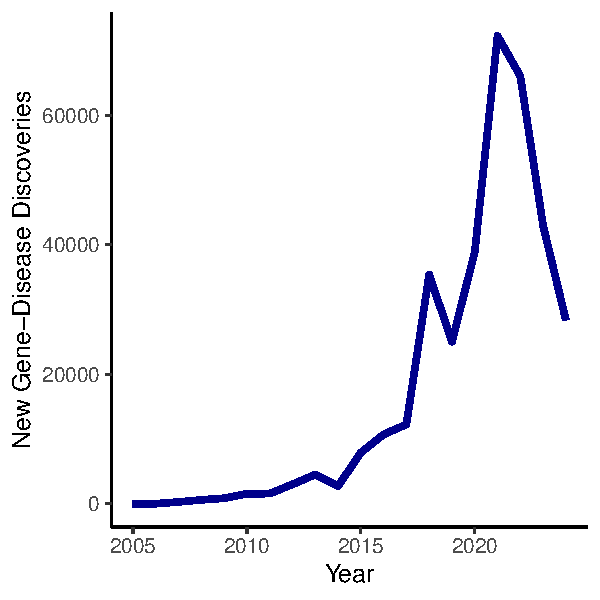
\includegraphics[width=.4\linewidth]{figures/discovery_over_time.pdf}
\end{lightfigure}

The GWAS catalog only reports the disease and/or trait that a particular study is concerned with, so to match these data to Pharmaprojects, we need to make a correspondence between disease/traits and therapeutic class. We create two lists of the 200 distinct therapeutic class names and 28,540 disease names from GWAS. We then wrote a Python script that looped through each disease name and used OpenAI's GPT-4.0 API to identify any and all (at most three) corresponding therapeutic class names. We matched 22,381/28,840 disease names to 179/200 therapeutic classes. Then, for each therapeutic class--year, we count the number of new discoveries in corresponding diseases published in GWAS in that year. As Figure \ref{fig:discovery_over_time} shows, the coverage of GWAS is considerably weaker for the first three-quarters of our sample period (GWAS was only founded in 2008, after all). Consequently, we have a measure of discovery for 811 out of 2791 market observations. After dropping observations where we don't have an ATC-1 code, this becomes 809. 


\section{Results}\label{sec:results}

%% brief overview of how the the results are organized

We present our results in four parts. First, we provide correlational evidence for the three propositions derived from our model. We then discuss alternative explanations and how we deal with them. Third, we present various additional robustness analyses. Lastly, we explore which firms are more likely to launch multiple experiments, and which firms try novel approaches.

%%-------------------------------------------------------------
%%
%%
%%
%% [SUBSECTION] BASELINE CORRELATIONAL RESULTS
%%
%%
%%
%%-------------------------------------------------------------

\subsection{Diversity of Approaches and the Success of Experimentation}


We begin by examining, correlationally, the relationships theorized by Propositions 1 and 2 between experimenter scale, the diversity of approaches, and the average success of experimentation. We estimate the following econometric specification:


\begin{equation}
\label{eq:baseline_model}
\begin{aligned}
        y_{i, t} = \alpha + \beta_1{x_{i, t}} + \theta_{i, t} + \gamma_i\times\tau_t + \epsilon_{i, t}
\end{aligned}
\end{equation}

Where $y_{i, t}$ represents the market-year level dependent variable \emph{Target Diversity}, or \emph{Share of Pre-Clinical Success}. and $x_{i, t}$ is the average experimenter scale in a therapeutic class--year. We test this specification with and without $\theta_{i, t}$, which is our set of market structure control variables for the number of firms, targets, and pre-clinical experiments within a therapeutic class–year. In all models we include ATC-1$\times$Year fixed effects $\gamma_i\times\tau_t$, amd standard errors are clustered at the ATC-1 level to account for correlations in errors among market observations within the same industry group.

\begin{table}[h!]
    \centering
    \scriptsize
    \caption{\textsc{The market-level relationship between experimenter scale, the diversity of approaches, and success}}
    \vspace{1em}
        \input{tables/featured/all-props-baseline-correlations}

    \label{tab:baseline-regressions-all-props}
    \vspace{1em}
    \caption*{\scriptsize\emph{Notes:} This Table reports baseline regression results testing each Proposition. In columns (1) and (2), we test Proposition \ref{prop:model-choice} by regressing \emph{Target Diversity} on \emph{Average Experimenter Scale}, where the difference between the two models is that column (2) includes the set of \emph{Market Structure Controls}. \emph{Target Diversity} is the Shannon entropy of the relative abundance of targets employed in pre-clinical experiments, and \emph{Average Experimenter Scale} is the average number of pre-clinical experiments started by firms in a therapeutic class--year. In columns (3) and (4), we test Proposition \ref{prop:model-outcomes} by regressing the \emph{Share of Pre-Clinical Success} on \emph{Average Experimenter Scale}. Lastly, columns (5) and (6) correspond to Proposition \ref{prop:atleastone}, where we explore the relationship between \emph{Target Diversity} and \emph{At least 1 Pre-Clinical Success}. All models are estimated with OLS. Robust standard errors clustered at the ATC-1 level are shown in parentheses. Significance codes: * p<.1, ** p<.05, *** p<.01 }
\end{table}

We present the results from this baseline specification in Table \ref{tab:baseline-regressions-all-props}. Column (1) reports the baseline relationship between experimenter scale and target diversity, showing a positive and significant association. In column (2), we incorporate market structure controls. Notably, the estimated coefficient for $\beta_1$ remains consistent across models. Based on the estimate in column (2), our findings suggest that a 1-unit increase in the average experimenter scale (e.g., from an average of 1.1 to 2.1 experiments per firm) corresponds to a 1.65 standard deviation increase in target diversity, which is consistent with Proposition \ref{prop:model-choice}.

In columns (3) and (4) we test Proposition \ref{prop:model-outcomes}: small-scale experimenters are more likely to be successful in an individual experiment than large-scale experimenters. Here we regress the \emph{Share of Pre-Clinical Success} on \emph{Average Experimenter Scale}, and find a negative relationship, consistent with our prediction. 

Lastly, to test Proposition \ref{prop:atleastone} we estimate the specification detailed in Equation \ref{eq:baseline_model} where the independent variable $x_{i, t}$ is \emph{Target Diversity} and the dependent variable $y_{i, t}$ is \emph{At least 1 Pre-Clinical Success}. The results are presented in columns (5) and (6) of Table \ref{tab:baseline-regressions-all-props}. Consistent with Proposition \ref{prop:atleastone}, these results indicate that markets with greater approach diversity in experimentation have a higher probability of at least one success. 


\begin{figure}[h!]
\caption{\textsc{Binned scatter plots of the market-level relationship between experimenter scale, the diversity of approaches, and success}}
\label{fig:baseline-nonparametrics}
    \centering
    \begin{subfigure}[t]{.3\textwidth}
        \centering
        \caption{Target Diversity}
        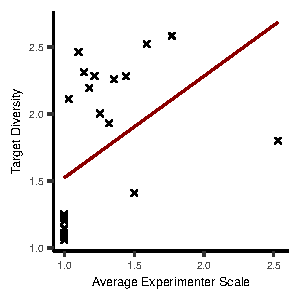
\includegraphics[width=\linewidth]{figures/featured/target_diversity_exp_scale.pdf}
    \end{subfigure}
    \begin{subfigure}[t]{.3\textwidth}
        \centering
        \caption{Average Success}
        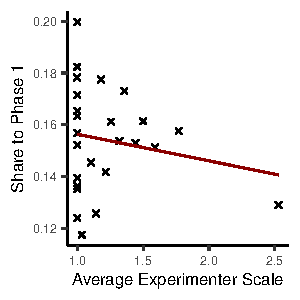
\includegraphics[width=\linewidth]{figures/featured/scale_phase1_share.pdf}
    \end{subfigure}
        \begin{subfigure}[t]{.3\textwidth}
        \centering
        \caption{At least one success}
        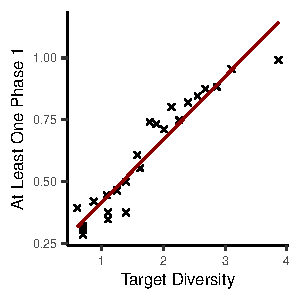
\includegraphics[width=\linewidth]{figures/featured/diversity_atleastone_phase1.pdf}
    \end{subfigure}
\caption*{\scriptsize\emph{Notes:} This Figure shows non-parametric binned scatter plots of the relationship between \emph{Target Diversity}, \emph{Average Experimenter Scale}, the \emph{Share of Pre-Clinical Success}, and \emph{At least 1 Pre-Clinical}, corresponding to the parametric estimates in Table \ref{tab:baseline-regressions-all-props}. Each plot uses 25 bins. }
\end{figure}

%%-------------------------------------------------------------
%%
%%
%%
%% [SUBSECTION] ALTERNATIVE EXPLANATIONS
%%
%%
%%
%%-------------------------------------------------------------
\subsection{Alternative Explanations}

Establishing causality in this context is challenging. The ideal experiment would involve identifying a source of exogenous variation in the cost or value of experimentation for certain firms in a market. For instance, a reduction in the cost of experimentation for some firms within a market could lead to an increase in the number of experiments they initiate, thereby altering the average experimenter scale without directly affecting the diversity of approaches used. While shocks that influence entire markets do exist---for example, the introduction of Medicare Part D in 2004, which arguably increased the value of experimentation in therapeutic classes with predominantly elderly patients \citep{dranove2022does}---such shocks tend to affect \emph{all} firms operating in the market.\footnote{One possible refinement could consider the geographic dimension of drug development. Since Medicare Part D was enacted in the U.S., its impact may have been limited to U.S. pharmaceutical firms within relevant therapeutic classes. However, because pharmaceutical companies operate globally, they are unlikely to be geographically isolated. Moreover, a shock like Medicare Part D could produce mixed effects. While it might encourage firms previously conducting only one experiment to initiate two, it could also incentivize new market entry, enabling firms that otherwise would not have participated to conduct experiments. Consequently, the impact on the composition of the experimenter scale within a market remains ambiguous.}

Instead, we take a multipronged approach to evaluate alternative explanations that would undermine our results. Our strongest argument is that neither alternative explanations nor likely sources of unobserved heterogeneity can explain the pattern of empirical results regarding the success of experimentation (Propositions \ref{prop:model-outcomes} and \ref{prop:atleastone}):  that greater experimenter scale increases the probability of at least one success but lowers average success. If the relationship between the average experimenter scale and target diversity were driven solely by unobserved common variables, we would not expect higher target diversity to correlate with both a higher probability of at least one success and a lower average share of successes in the market. 

For instance, suppose that some markets have more technical opportunities, and this is positively (negatively) associated with the number of approaches observed. Then, there should be a positive (negative) relationship between diversity and average success but also at least one success. There is no reason to expect a relationship between diversity and average size. Alternatively, suppose, for some reason, experimenter-scale is positively related to technological opportunity, which, in turn, is positively related to the diversity of approaches. This would result in a positive association between experimenter-scale and diversity. However, this should also increase, not decrease, average success. Thus, while we cannot establish a causal link between experimenter scale and target diversity, the observed associations between experimenter scale, target diversity, and success outcomes are consistent with the hypothesized causal relationship.

\begin{table}[h!]
    \centering
    \scriptsize
    \caption{\textsc{Linking approach diversity to the success of experiments}}
    \label{tab:linking-diversity-to-success}
    \vspace{1em}
        \input{tables/featured/link-diversity-to-success}
    \vspace{1em}
    \caption*{\scriptsize\emph{Notes:} This Table reports regression results that link success outcomes to the diversity of targets, while controlling for the average scale of experimenters in the market. In column (1), we regress \emph{Share of Pre-Clinical Success} on  \emph{Target Diversity}, and in column (2) we include \emph{Average Experimenter Scale} as a control. Columns (3) and (4) are similar, but the dependent variable is \emph{At least 1 Pre-Clinical Success}. All models are estimated with OLS. Robust standard errors clustered at the ATC-1 level are shown in parentheses. Significance codes: * p<.1, ** p<.05, *** p<.01 }
\end{table}


%%--- other controls
There are some possible confounding variables which we can observe and directly control for. The first concerns the discovery of new targets. Our model and simulations assume a fixed pool of approaches from which firms select for experimentation, but the landscape of available approaches may evolve over time. The discovery of new targets and their relationships with therapeutic indications could expand the pool of available approaches, naturally increasing target diversity. Additionally, this dynamic could influence the composition of experimenter scale in the market if single- or multi-experiment firms differ in their likelihood of introducing novel targets.

Second, there could be underlying average firm characteristics within a market that are correlated with both the number of experiments firms' choose to launch and their choice of approach. For instance, younger firms may be less likely to conduct multiple experiments due to limited resources to fund and manage them. Additionally, if younger firms are more inclined to pursue novel approaches, the average firm age in a market could be correlated with target diversity.

In Table \ref{tab:all-props-baseline-with-controls}, we replicate the analysis from Table \ref{tab:baseline-regressions-all-props}, adding controls for discovery and average firm age. In column (1), the coefficient on \emph{Average Experimenter Scale} increases in magnitude when $\ln(Discovery)$ is included compared to the baseline result in column (1) of Table \ref{tab:baseline-regressions-all-props}, suggesting that the baseline model may underestimate the effect due to a downward bias. However, these results are limited by a smaller sample size, stemming from challenges in mapping new target discoveries to therapeutic classes. In column (2), which includes only the control for average firm age, the coefficient remains consistent with the baseline results reported in column (3) of Table \ref{tab:baseline-regressions-all-props}. Using the estimate from the full model in column (3), we find that a 1-unit increase in the average experimenter scale is associated with a 1.38 standard deviation increase in target diversity, slightly smaller than the baseline result.

As for the average success of experimentation, the inclusion of our control for discovery supresses the negative relationship reported between \emph{Average Experimenter Scale} and \emph{Target Diversity}. Still, after controlling for discovery we find no relationship between average exeperimenter scale and average success. Note that in column (5), which only includes the control for average firm age, the estimated coefficient is indistinguishable from the baseline estimate in column (4) of Table \ref{tab:baseline-regressions-all-props}.

Lastly, column (7) through (9) report the relationship between diversity and at least one pre-clinical success after controlling for target discovery and average firm age. When $\ln(Discovery)$ is included, the estimated coefficient on \emph{Target Diversity} is marginally less than the baseline result in column (6) of Table \ref{tab:baseline-regressions-all-props}. This suggests that the baseline model may slightly overestimate the effect due to a upward bias. Yet, we still find a positive and statistically significant relationship between the diversity of targets and the likelihood of at least one pre-clinical success.


\begin{table}[h!]
    \centering
    \scriptsize
    \caption{\textsc{The relationship between experimenter scale and target diversity while controlling for target discovery and firm age}}
    \vspace{1em}
    \resizebox{\textwidth}{!}{
        \input{tables/featured/all-props-baseline-with-controls}
    }
    \label{tab:all-props-baseline-with-controls}
    \vspace{1em}
    \caption*{\scriptsize\emph{Notes:} This Table reports baseline regression results testing each Proposition while controlling for two observable potential confounders. In columns (1) through (3), we regress \emph{Target Diversity} on \emph{Average Experimenter Scale}. Column (1) includes \emph{ln(Discovery)}, column (2) includes \emph{Average Firm Age}, and column (3) includes both variables. Recall that \emph{ln(Discovery)} is the natural logarithm of the count of publications in GWAS that report a novel target, and \emph{Average Firm Age} is the average age of distinct experimenters (firms) in a therapeutic class--year. The remaining models follow the same pattern, where the dependent variable in columns (4) through (6) is \emph{Share of Pre-Clinical Success}, and in columns (7) through (9) the dependent variable is \emph{At least 1 Pre-Clinical Success}. Note that in the final three columns---consistent with the baseline results in Table \ref{tab:baseline-regressions-all-props} that test Proposition \ref{prop:atleastone}---the indepednent variable of interest is  \emph{Target Diversity}. All models are estimated with OLS. Robust standard errors clustered at the ATC-1 level are shown in parentheses. Significance codes: * p<.1, ** p<.05, *** p<.01}
\end{table}



\begin{table}[h!]
    \centering
    \scriptsize
    \caption{\textsc{Alternative Explanations}}
    \label{tab:alternative-explanations}
    \vspace{1em}
        \input{tables/featured/alternative-explanations} 
    \vspace{1em}
\end{table}



\begin{comment}
refer to emily oster approach that considers size of coefficient change
\end{comment}



%%-------------------------------------------------------------
%%
%%
%%
%% [SUBSECTION] ROBUSTNESS
%%
%%
%%
%%-------------------------------------------------------------

\subsection{Robustness}

We also subject our baseline results to a series of robustness tests. The first addresses the complication that arise when a target is known to be a valid approach. In our model, this corresponds to an approach where $\pi$—the probability that the approach is a viable solution to the problem—equals one, meaning there is \emph{no} uncertainty about its viability. When $\pi=1$, the key implication is that outcomes for experiments using the same approach are no longer correlated, as success depends solely on implementation (see Appendix \ref{app:proofs}). In this case, firms will naturally select the approach with they have the highest probability of implementation success. We restrict the underlying project-level dataset to projects where the target chosen has not been successfully drugged, which we measure by the first launched product. In Appendix Table \ref{app:drop_pi_equal_one}, we replicate our core results in Table \ref{tab:baseline-regressions-all-props}, and find quantitatively similar estimates.

Second, we test the sensitivity of our results to alternate time windows. The unit of analysis in our baseline results is the therapeutic class--year. The choice to look within a single year is arbritary, so we construct two additional datasets, where we define observations within a two-year and five-year window. Table \ref{app:longer_time_windows} in the Appendix reports these results. Although we lose the number of observations through a higher level of aggregation, we find results consistent with our preferred specification which defines observations within a 1-year period. The only exception is that we lose statistical signficance between average experimenter scale and average success in the therapeutic class--five year period data, and find no relationship instead.

Third, we explore the robustness of our results to alternate measures of key variables. In particular, we test the sensitivity of our results to measuring target diversity with the Herfindahl-Hirschman Index. We also test an alternative measure to success, where we define success as whether a pre-clinical experiment ultimately results in a drug product launch. Table \ref{app:alternative_measures} in the Appendix shows results qualitatively similar to our baseline finding with these alternative measures.

Lastly, we attempt to address possible simultaneity bias by leveraging the panel structure of our data. Specifically, we use the average experimenter scale in the previous year $(i, t-1)$ as an instrument for the average experimenter scale in year $t$. This instrument relies on the assumption that idiosyncratic factors, unrelated to target diversity or underlying success probabilities, drive some markets to have more firms with lower experimentation costs. If these factors are persistent, the lagged experimenter scale would be correlated with the current experimenter scale but would not capture time-varying unobserved variables that influence experimenter-scale and target diversity.\footnote{Using the lagged experimenter scale as an instrument helps address simultaneity bias, but it cannot fully account for unobserved, market-specific and time-persistent factors---such as market dynamics, innovation strategies of firms, or public research funding across markets ---that may influence both experimenter scale and target diversity. However, our results are robust to controlling for aggregate industry-level time trends, captured by ATC-1$\times$Year fixed-effects  \citep{branstetter2022generic}.} We find, as described in Appendix Table \ref{app:2sls}, that the relationship between target diversity and experimenter-scale is strengthened.


%%-------------------------------------------------------------
%%
%%
%%
%% [SUBSECTION] WHICH FIRMS DO WHAT?
%%
%%
%%
%%-------------------------------------------------------------

\subsection{Which firms do multiple experiments and introduce novelty?}\label{subsec:which-firms}

Our data and results raise at least two questions, which we explore in this section. First, we have not addressed which firms choose to launch multiple experiments. One potential mechanism, demonstrated in our simulations, involves exogenously shifting the share of multi-experiment firms by altering the proportion of firms facing high or low experimentation costs. Alternatively, the same outcome could be achieved by allowing some firms to extract greater value from experiments, prompting them to enter with additional experiments.

A large body of research in Strategy and Economics suggests that firm size likely explains this pattern. Specifically, multi-experiment firms are most likely \emph{large}, as they benefit from lower experimentation costs \citep{cohen1996reprise} and can appropriate greater value from experiments \citep{arora2023invention}. This advantage stems, in part, from their complementary downstream co-specialized assets, which are essential for commercialization \citep[e.g.,][]{rosenbloom2000leadership, filippetti2017appropriability}.

We use firm ownership as a proxy for firm size, distinguishing between private and public firms. Interestingly, the data provide no evidence that public firms are more likely to conduct multiple experiments in a market. In panel (a) of Figure \ref{fig:firm-heterogeneity}, we show that private firms conduct only one experiment in a therapeutic class–year 61.5\% of the time. For public firms, this share is slightly \emph{higher}, at 63.3\%. Panel (b) presents the raw counts of experiments by experimenter scale. While public firms conduct significantly more experiments overall, the data reveal that, most of the time, they launch only one pre-clinical experiment in a therapeutic class–year.


Second, considering the discovery of new targets adds an intriguing nuance: which firms are more likely to introduce novelty? Specifically, when a new target–therapeutic class link is discovered, which firms—if any—are more likely to be the first to pursue this approach in pre-clinical trials? In panel (c) of Figure \ref{fig:firm-heterogeneity}, we plot the share of experiments by single-experiment firms and multi-experiment firms (those conducting more than one experiment in a therapeutic class–year) that are the first to use a target in a therapeutic class.

To ensure reliability, we include only projects initiated since 2005, as earlier projects are more likely to represent the first target–therapeutic class combinations due to the dataset’s starting point in 1995, which excludes targets drugged before this year. Panel (c) shows that single-experiment firms are more likely to drug a novel target: 54.9\% of experiments by these firms introduce a new target, compared to 45.9\% for multi-experiment firms. However, panel (d) reveals no significant difference between private and public firms in their likelihood of targeting a novel approach.

These results highlight a critical trade-off in the optimal allocation of experiments within a market. Markets dominated by small-scale experimenters are less favorable for innovation in some respects, as they are more likely to rely on a less diverse set of approaches and are less likely to achieve at least one successful experiment. However, these markets are also more likely to introduce new targets, drugging them for the first time.

\begin{figure}[h!]
\caption{\textsc{The relationships between ownership, experimenter scale, and the likelihood of experimenting with novel targets}}
\label{fig:firm-heterogeneity}
    \centering
    \begin{subfigure}[t]{.24\textwidth}
        \centering
        \caption{}
        \includegraphics[width=\linewidth]{figures/private_public_same_scale.pdf}
        \label{subfig:private_public_same_scale}
    \end{subfigure}
    \begin{subfigure}[t]{.24\textwidth}
        \centering
        \caption{}
        \includegraphics[width=\linewidth]{figures/count_exp_obs_public_private.pdf}
        \label{subfig:count_exp_obs_public_private}
    \end{subfigure}
    \begin{subfigure}[t]{.24\textwidth}
        \centering
        \caption{}
        \includegraphics[width=\linewidth]{figures/singles_more_discovery.pdf}
        \label{subfig:singles_more_discovery}
    \end{subfigure}
        \begin{subfigure}[t]{.24\textwidth}
        \centering
        \caption{}
        \includegraphics[width=\linewidth]{figures/private_public_discovery.pdf}
        \label{subfig:private_public_discovery}
    \end{subfigure}
\caption*{\scriptsize\emph{Notes:} This figure explores the non-parametric relationships between ownership, experimenter scale, and the likelihood of experimenting with novel targets. The data for all panels only includes projects from 2005 and onwards. This is to address the concern that novelty may be artificially inflated in earlier years because our data starts in 1995, and novelty is defined with respect to what came before. Panel (a) is a bar chart comparing the average share of private and public firms that conduct multiple experiments in a therapeutic class--year. Panel (b) plots the count of experiments conducted by experimenter scale for both public and private firms. Panel (c) compares the share of experiments conducted by multi-experiment and single-experiment firms that use a novel target. Panel (d) compares the share of experiments conducted by private and public firms that use a novel target. 
}
\end{figure}




\section{Discussion}

This paper addresses the question of how market structure influences the diversity of experimental approaches firms take and, ultimately, the likelihood of solving innovation problems with uncertain solutions. To investigate this, we develop a theoretical model that builds on work by \citet{dasgupta1987simple} and \citet{bryan2017direction} that explores how firms choose between approaches under varying market structures, focusing on multi-experiment firms versus single-experiment firms. The model yields three key propositions at the market level. First, firms conducting multiple experiments are more likely to diversify their approaches, whereas many single-experiment firms tend to converge on the most promising approach, reducing market-level diversity. Second, markets dominated by single-experiment firms achieve higher success rates per experiment, due to their focus on the most promising approach. Third, multi-experiment firms maximize the probability of at least one success through diversification, implying that markets with greater experimenter scale are more likely to see at least one experimental success. To test these propositions, we use detailed data on early-stage pharmaceutical drug development, spanning 49,866 projects across 27 years, and demonstrate how experimenter scale drives approach diversity and influences market-level success.

The findings reveal a robust and significant relationship between experimenter scale and approach diversity. Markets with a higher average experimenter scale---where firms conduct multiple experiments---exhibit a nearly three standard deviation increase in target diversity for every one-unit increase in average scale. This effect is consistent across alternative econometric specifications. Importantly, markets with higher experimenter scale are more likely to achieve at least one successful outcome, with a one-unit increase in scale linked to a 25.9 percentage point rise in the likelihood of at least one experiment progressing to Phase 1 trials. However, this benefit comes at the cost of a lower average success rate per experiment, as larger-scale experimentation dilutes focus on the most promising approaches. Consequently, we also see that markets with greater approach diversity---driven by multi-experiment firms---are more likely to achieve at least one successful outcome, compared to markets dominated by single-experiment firms. These results are robust to alternative explanations, including controls for new target discovery and firm age, underscoring the role of multi-experiment firms in fostering a diverse innovation ecosystem while balancing trade-offs in efficiency and exploratory breadth. 

Our findings have implications for the broader literature on experimentation and innovation. By highlighting the dual roles of small- and large-scale experimenters, we add to the understanding of how diversity in approaches arises and evolves within markets \citep{cohen1992tradeoff}. Small-scale experimenters act as pioneers, introducing novel approaches that expand the frontier of possibilities, while large-scale experimenters provide depth by thoroughly testing and validating established approaches \citep{kotha2011entry, ahuja2001entrepreneurship}. This complementarity bridges gaps in the literature on technological trajectories, suggesting that innovation ecosystems benefit from balancing exploratory breadth with systematic refinement \citep{luger2018dynamic, fang2010balancing, chen2008rival}. Our distinction between approach and implementation further informs studies of experimentation by underscoring how shared risks in approach viability can amplify herding behaviors and potentially limit diversity in high-stakes contexts.

For policy, our results suggest a nuanced perspective on fostering innovation through experimentation. Encouraging both small- and large-scale experimenters within markets is crucial to achieving a balance between exploration and exploitation. Policies that support small-scale experimenters, such as grants for early-stage research or incubator programs, can help uncover novel targets and approaches \citep{bradley2021policy}. Meanwhile, mechanisms that enable larger firms to scale their experimentation, such as tax incentives or public-private partnerships, ensure that promising but understudied approaches receive the rigorous testing needed for broader application \citep{dimos2016effectiveness, lerner2009boulevard}. By designing interventions that maintain this balance, policymakers can enhance the robustness of innovation ecosystems and increase the likelihood of market-level breakthroughs.

These insights also have practical implications for the structure of research funding and the design of innovation ecosystems. Allocating resources to create spaces where small-scale experimenters can explore untested ideas while facilitating partnerships with larger organizations can improve innovation outcomes \citep{cappelen2012effects}. For instance, collaborative frameworks that combine the agility of startups with the resources of established firms may foster a more diverse and productive experimental landscape \citep{polidoro2021corporate, bhaskaran2009effort}. Similarly, strategies that mitigate herding, such as incentivizing exploration of high-risk, high-reward approaches, can prevent over-concentration on seemingly safe options, thus ensuring a more resilient innovation pipeline \citep{von2020exploration}. Together, these findings offer actionable pathways to strengthen the interplay between individual and collective experimentation in driving technological and societal progress.

While our findings provide valuable insights, several limitations warrant discussion. First, the causal interpretation of our results remains challenging. Although we use extensive controls, unobserved factors—such as market-specific shocks to funding, technology, or regulation—may bias our estimates. For example, simultaneous drivers of experimenter scale and diversity, like regulatory changes or scientific breakthroughs, complicate causal attribution. However, such factors are unlikely to account for the full set of empirical associations we document.

Second, our focus on the pharmaceutical industry, while offering rich data, limits generalizability. Pharmaceuticals involve high R\&D costs, long timelines, and significant uncertainty, which may amplify the dynamics we observe. Other industries, with different innovation cycles or competitive pressures, might display distinct patterns. Exploring these relationships in contexts like materials or renewable energy could test the broader applicability of our model and findings. However, we believe this limitation applies primarily to the empirical setting, not the underlying theory. With regard to our theory, our assumptions enforce two key scope conditions: (1) the total value from experimentation is fixed and independent from the \emph{number} of successes, and (2) that there is variation across firms in their ability to conduct multiple experiments. At first, these scope conditions may seem restrictive, but we believe that there are many markets and technologies---such as batteries, quantum computing, and medical devices---which look this way. In these industries, among others, experimentation is costly, which is one reason for variation in experimenter scale. Furthermore, all of these examples share the promise of temporary monopoly rents---that the first success will capture all value for a period of time.

Finally, deeper exploration of mechanisms and firm heterogeneity is needed. We highlight the roles of small- and large-scale experimenters but do not fully unpack how firm size, resources, or market structures influence their contributions to diversity and innovation. Future research should examine how these dynamics vary across industries and firm types, offering richer insights into the optimal design of innovation ecosystems.

By studying how market structure shapes collective experimentation outcomes, we hope this work encourages further analysis of how innovation systems can be designed to solve the complex and pressing problems.

\clearpage 

\footnotesize
\singlespacing
\bibliography{biblio}
\bibliographystyle{apalike}


\processdelayedfloats %printing tables and figures

\clearpage
\normalsize
\doublespacing

% \setcounter{page}{1}
\counterwithin{table}{section}
\vspace*{2cm}

\begin{center}
    \textbf{\Large Appendix:} 
    \\
    \Large If you had only one shot: Scale and herding in innovation experiments
\end{center}

\clearpage

\renewcommand{\thesection}{\Alph{section}}
\counterwithin{lightfigure}{section}
\counterwithin{lighttable}{section}

\appendix

\renewcommand{\thesection}{\Alph{section}}
\counterwithin{lightfigure}{section}
\counterwithin{lighttable}{section}

% Appendix content
\section{A Case Study on Approaches to Experimentation: Psoriasis}\label{app:case-study}

Psoriasis\footnote{https://www.niams.nih.gov/health-topics/psoriasis} is a chronic inflammatory skin condition affecting approximately 2-3\% of the global population \citep{Ayala-Fontanez}. A common symptom of the disease is the appearance of raised, silvery plaques \citep{Nestle-psoriasis}. Although treatments for psoriasis have been available for decades, the disease has many forms, and the causes of some less common types are still not fully understood \citep{guo2023signaling}. Many hypotheses exist, and some examples include: (i) overactive T-cells triggering inflammation and rapid skin cell production, (ii) genetic factors, such as mutations in the HLA-Cw6 gene, (iii) involvement of cytokines like IL-23 and IL-17, (iv) inflammatory lipid molecules called leukotrienes, and (v) abnormalities in keratinocytes that result in excessive skin cell production. This section describes examples of firms initiating pre-clinical trials for two distinct psoriasis drug development projects within the same year. These examples are sourced directly from Pharmaprojects and supplemented with details from Trialtrove.


\textbf{Astrazeneca.} In 2004, AstraZeneca began preclinical trials for two psoriasis treatments. One was a humanized antibody called Sifalimumab, which targeted interferon-alpha (IFN-$\alpha$). The underlying hypothesis was that in genetically predisposed individuals, the immune system is primed, and exogenous IFN-$\alpha$ may trigger psoriasis development.

At the same time, pre-clinical trials began for Certolizumab pegol, a recombinant humanized high-affinity anti-TNFalpha antibody fragment, developed by UCB (Celltech before the acquisition), for the treatment of chronic inflammatory conditions, including Crohn's disease (CD), rheumatoid arthritis (RA), psoriatic arthritis and ankylosing spondylitis 

The anti-TNF alpha psoriasis hypothesis suggests blocking Tumor Necrosis Factor-alpha (TNF-alpha). It has since been shown, however, that this approach can lead to the development or worsening of psoriasis, primarily due to an uncontrolled increase in type 1 interferons produced by plasmacytoid dendritic cells (pDCs), which are key players in psoriasis pathogenesis. 


\textbf{Stiefel Laboratories (GlaxoSmithKline).} In 2006, Stiefel Laboratories began pre-clinical trials for two psoriasis drugs. One was called Primolux, which was a 0.05\% topical formulation of the corticosteroid clobetasol, developed using its proprietary VersaFoam-EF technology, that targeted the nuclear receptor subfamily 3 group C member 1.

The second drug, Calcipotriol VersaFoam, was a vitamin D receptor antagonist. The treatment consisted of a 0.005\% topical formulation of calcipotriol, a vitamin D3 analog.

In 2009, GlaxoSmithKline acquired Stiefel Laboratories for \$2.9 billion to create a specialists dermatogolgy branch.\footnote{https://www.gsk.com/en-gb/media/press-releases/glaxosmithkline-completes-acquisition-of-stiefel} Consequently, in Pharmaprojects these projects are described as being originated by GlaxoSmithKline. This example highlights the complications in measurement. Pharmaprojects assigns the ``company developing a drug'' to each drug--treatment. Importantly, this would suggest that the listed focal company is both funding development and the primary decision maker.

Identifying the impact of such measurement error is hard to do. In the example of Stieffel laboratories, this measurement error would not affect ecometric estimates in our core results, at least. We would still consider the experiments to be done by a multi-experiment firm. If, however, we are on average more likely to incorrectly assign multi-experiment status to a large incumbent such as GlaxoSmithKline, then our analysis in Section \ref{subsec:which-firms} may inaccurately estimate the relationship between ownership type, the scale of experimentation, and the introduction of novelty (Figure \ref{fig:firm-heterogeneity} panels (a), (b), and (d)) 

However, measurement error in general would create an attenuation bias. In particular, if measurement error is also correlated with the target diversity dependent variable. If firm $X$ acquired two single experimenters, each with a distinct approach, and both experiments are attributed to firm $X$, then this would be a positive correlated measurement error leading to an upward bias on the estimated coefficient. Given our data, it is not feasible to scrutinize the history of each drug development project and the accuracy of originator firm assignment. This should be recognised as an empirical limitation of this study.
\clearpage
\section{Model Extensions}\label{app:proofs}

While simulations are best suited to generalizing our model, we can formally extend the model to analyze the decision of the $n^{th}$ experiment after $n-1$ experiments in approach $a$. For simplicity, we set $\pi_a = \pi_b = \pi$. Instead, approach $a$ is assumed to be more promising than $b$ because $p_a > p_b$ for all experimenters.

In addition, we relax our rent-sharing assumption. In the baseline model in the two-firm case, we assume that if both experiments are successful, only one experiment will capture value (with probability 0.50). In this extension, we consider the scenario where the probabilities of value capture can be lower. Concretely, this permits the scenario where two firms are successful, and they can both commercialize their innovations, but due to competition, the value they capture is less than $V/2$. We model rent dissipation with the parameter $k$ to analyze the effect of rent dissipation on the choice of approach.

%%%%%%%%%%%%%%%%%%%%%%%%%%%%%%%
%% competition/multiple entries
%% The choice of approach with $N$ periods and rent dissipation.
%%%%%%%%%%%%%%%%%%%%%%%%%%%%%%%

Suppose there are $n$ firms and $n$ experiments in approach $a$ and 0 experiments in $b$, such that each firm is a single-experiment firm. A potential entrant in approach $a$ has a payoff of:
\begin{equation} \label{eq: n in A A}
\begin{aligned}
    &p_a \pi \left((1-p_a)^n + \frac{1}{2+k}{n \choose 1}a(1-p_a)^{n-1} +\frac{1}{3+k}{n \choose 2}(p_a)^2(1-p_a)^{n-2} ... \frac{1}{n+1 + k}(p_a)^n \right) -c  \\
    &= p_a \pi X(n,k) - c
\end{aligned}
\end{equation}
Note that $X(n,k)$ is strictly less than unity, and decreases with the rent dissipation parameter $k$, because each of the terms $\dfrac{1}{n+1_k}p_a^n$ decreases with $k$. Note also that $X(n,k) - (1-p_a)X(n-1,k)$ is positive but falls with $k$. Formally,

\begin{equation} 
\begin{aligned}
&X(n,k) - (1-p_a)X(n-1,k) = \\
&\frac{1}{2+k}\left({n \choose 1}-{n-1 \choose 1}\right)a(1-p_a)^{n-1} + 
\frac{1}{3+k}\left({n \choose 2}-{n-1 \choose 2}\right)p_a^2(1-p_a)^{n-2} \\
&.. + \frac{1}{n+k}(p_a)^n > 0
\end{aligned}
\end{equation}
That $X(n,k) - (1-p_a)X(n-1,k)$ decreases with $k$ follows upon noting that each terms, $\frac{1}{r+k}\left({n \choose r-1}-{n-1 \choose r-1}\right)p_a^{r-1}(1-p_a)^{n-1 - (r-1)}$, decreases with $k$.

\subsection{Incentives to herd and scale of experimentation}
\noindent Entering $b$ instead has a payoff of:
\begin{equation} \label{eq: n in A B}
    p_b \pi \left(\pi X + (1-\pi)\right) = p_b\pi^2 X(n,k)  + p_b \pi(1-\pi) -c
\end{equation}

\noindent The incentive to herd into approach $a$ for the single-experiment entrant is given by:
\begin{equation}\label{eq herd small n}
 \Delta_s =  \pi(p_a-\pi p_b)X(n, k) + \pi(1-\pi p_b)
\end{equation}


\noindent Now consider a potential multi-experiment firm, which has one experiment in $a$ along with $n-1$ other firms i.e., an incumbent. The payoff to this firm of a second experiment in $a$ is:
\begin{equation} \label{eq: n in A A big}
\begin{aligned}
     &\pi(p_a(2-p_a) \left((1-p_a)^{n-1} + \frac{1}{2+k}{n-1 \choose 1}p_a(1-p_a)^{n-2} + ... \frac{1}{n + k}p_a^{n-1} \right) \\ 
     &=  \pi X(n-1,k)p_a(2-p_a) - c
\end{aligned}
\end{equation}
\noindent And their payoff from entering with approach $b$ is given by:
\begin{equation} \label{eq: n in A B }
\pi X(n-1,k)(a +\pi (1-a)b)+ b\pi(1-\pi)-c    
\end{equation}

\noindent Thus the incentive to herd in approach $a$ for the incumbent firm can be expressed:
\begin{equation}\label{eq herd large n}
   \Delta_M = \pi (1-p_a)X(n-1, k)(p_a-\pi p_b) + \pi (1-\pi)p_b
\end{equation}

\noindent It follows that $\Delta = \Delta_s - \Delta_M = \pi (1-\pi p_b) \left[X(n,k)-(1-p_a)X(n-1,k) \right] > 0$. That is, if the $(n+1)^{th}$ experiment is conducted by a new entrant, they will be more likely to experiment with approach $a$ compared to a multi-experiment firm who is incumbent with an existing experiment in approach $a$. Furthermore, $\Delta$ falls with $k$ because $X(n,k)-(1-p_a)X(n-1,k)$ falls with k. \textbf{That is, small-scale experimenters are more likely to herd than large-scale experimenters, but less so when rents are dissipated.}  


\begin{comment}
I commented this out because we do not have results about how crowded the approach is    
\end{comment}

\begin{comment}
This tendency is also reflected in how sensitive firms are to how crowded approach $a$ is. To see this, consider $n_L^*$ such that the incumbent firm is indifferent between entering $a$ or $b$, i.e.,  $n_L^*$ is implicitly defined by $(1-p_a)X(n_L^*-1) = \dfrac{(1-\pi p_b)}{(p_a- \pi p_b)}$. Because $X(n_L^*,k) > (1-a)X(n_L^*, K) = \dfrac{(1-\pi b)}{(a- \pi b)}$, $\Delta_s > 0$. \textbf{In other words, as the number of experiments in $a$ increases, the multi-experiment firm will switch to $b$ before a single-experiment entrant.}

We can obtain an analogous result for the attractiveness of the alternative approach $p_b$. Define a threshold value $p_b^*$ where a new entrant (single experimenter) is indifferent between $a$ and $b$, so that $p_b > p_b^*$ implies that the entrant prefers to enter $b$.  The threshold is given by:  
\begin{equation} \label{eq: threshhold b*}
\begin{aligned}
p_b^*=\frac{p_aX(n,k)}{\pi X(n,k) + (1-\pi)} 
\end{aligned}
\end{equation}

Let $p_b^{**}$ be the threshold such that an incumbent (potential multi-experimenter) is indifferent between $a$ and $b$.  Then $p_b^{**}$ is given by   
\begin{equation}\label{eq: threshold b**}
    p_b^{**}=\frac{p_a(1-p_a)X(n-1,k)}{\pi(1-p_a)X(n-1,k) +(1-\pi)}
\end{equation}

\noindent Note that $p_b^* > p_b^{**}$ because $X(n,k) \geq (1-p_a)X(n-1,k)$. That is, the threshold value of $p_b$ such that the multi-experiment firm is indifferent between $a$ and $b$ is smaller than the single-experiment entrant. \textbf{For any given $a$, there is a range, [$p_b^{**}, p_b^{*}$], such that a multi-experiment firm would enter $b$ whereas a single-experiment firm would continue to herd in $a$.} 


Then we can specify the following facts about $b^*$:

\begin{itemize}
   \item $b^*$ increases with $X$, so that it decreases with $n$ \& $k$
   \item $b^*$ increases with $a$   %% \todo{check. X depends on a as well}
   \item $b^*$ increases with $\pi$ because $\pi X +1-\pi$ falls with $\pi$
\end{itemize}

In sum, because $b^*$ falls with $n$, as the number of experiments in an approach increase, future experiments are more likely to choose the other approach. Because $b^*$ increases with $\pi$, the switch happens faster when the approaches are less promising.     
\end{comment}


\clearpage
\section{Simulation}\label{app:simulations}

\subsection{Logic}

In the model developed in Section \ref{sec:model}, there are two important assumptions underlying its basic intuition. First, the total value that can be captured by successful firms is independent of the number of successful firms - meaning the total profit from successful experiments by independent firms stays constant. Specifically, a firm with two successful experiments earns the same payoff as if it had only one successful experiment. This implies that competition among successful firms does not dissipate rents but merely distributes the total payoff in some fashion. The second assumption is that the validity of approaches is uncertain. Firms choosing the same approach are more likely to succeed or fail together than firms choosing different approaches, meaning value diversion is more likely when firms choose the same approach. In other words, firms choosing the same approach have correlated outcomes, whose effect is not fully integrated into individual firms' decisions. However, this correlation arises only if $\pi \neq 1$; if $\pi = 1$, the probability of success depends solely on implementation. Thus, firms will choose the approach with which they have the highest probability of implementation success. Target diversity at the market level would simply reflect differences in implementation ability for different approaches.

Generalizing beyond two approaches and two possible experiments to multiple approaches and multiple firms involves considerations of competition and order of entry into experimentation. While this is not analytically tractable, simulations permit us to explore the robustness of the model's intuition. We use Monte Carlo simulations to generalize the results of our model. In the baseline simulation, we define a pool of 50 firms, of which $\phi \in[0,1]$ have a high cost of experimenting (and $1-\phi$ incur a low cost). In each period, a firm is randomly selected and can choose to experiment. Firms experiment with the approach that returns the largest non-negative expected payoff and do not enter if all expected payoffs are negative. This payoff depends on the ongoing experiments and whether the firm has an ongoing experiment. Once a firm has entered twice we remove them from the pool of firms. We run simulations for different shares $\phi$ to exogenously create variation in the share of firms that enter with two experiments (a higher share of high-cost firms leads to fewer firms entering with two experiments). A simulation ends when the first low-cost firm chooses not to enter since this indicates that there will be no more entry (high-cost firms are less likely to enter than low-cost firms, given their higher cost). We run 400 simulations for $\phi = \{0, 0.1, 0.2, 0.3, 0.4, 0.5, 0.6, 0.7, 0.8, 0.9, 1\}$

Figure \ref{fig:simulations} presents results from the baseline simulation, where we simulate firms choosing between two approaches, $a$ and $b$, where $\pi_a < \pi_b$. Firms continue to enter until they become unprofitable with either approach. In panel \ref{subfig:sims_choice}, we link the market-level share of multi-experiment firms to the diversity of approaches used. Maximum diversity would be an even split between approach $a$ and $b$, with target diversity defined as one minus the share of experiments using approach $a$. Our simulations support the analytical prediction that greater approach diversity occurs when firms conduct multiple experiments on average. In panels \ref{subfig:sims_success_share} and \ref{subfig:sims_choice_to_outcomes}, we show results from simulations predicted by Propositions \ref{prop:model-outcomes} and \ref{prop:atleastone}. Markets with a greater share of multi-experiment firms have a lower individual experiment success rate. However, in markets with greater approach diversity---associated with more multi-experiment firms---we observe a higher probability of at least one experiment succeeding.

\begin{lightfigure}[h!]
\caption{\textsc{Simulation Results}}
\label{fig:simulations}
    \centering
    \begin{sublightfigure}[t]{.3\textwidth}
        \centering
        \caption{}
        \includegraphics[width=\linewidth]{figures/sims_choice.pdf}
        \label{subfig:sims_choice}
    \end{sublightfigure}
    \begin{sublightfigure}[t]{.3\textwidth}
        \centering
        \caption{}
        \includegraphics[width=\linewidth]{figures/sims_success_share.pdf}
        \label{subfig:sims_success_share}
    \end{sublightfigure}
    \begin{sublightfigure}[t]{.3\textwidth}
        \centering
        \caption{}
        \includegraphics[width=\linewidth]{figures/sims_choice_to_atleastone_successe.pdf}
        \label{subfig:sims_choice_to_outcomes}
    \end{sublightfigure}
\caption*{\scriptsize\emph{Notes:} These figures report binned scatter plots of our simulation results, illustrating the relationships predicted by each proposition. We simulate 1500 markets, creating variation in the share of large-scale experimenters by exogenously shifting the share of firms that have a high cost of experimenting. A detailed explanation of the simulation logic is provided in Appendix \ref{app:simulations}. This simulation uses the following parameters: $\pi_a = 0.4$, $\pi_b = 0.2$, $p_a = p_b = 0.3$.}
\end{lightfigure}

\subsection{Extension: Discovery of new Approaches}

A feature of our empirical context is that new approaches are discovered. Additionally, in practice, more than two approaches will be available to the experimenter. In our empirical context, for example, the average number of targets observed in a therapeutic class--year is 9.09 (median=5, std.dev.=14.21, min=2, max=210. Here, we extend our simulation framework to allow for discovery and, thus, multiple approaches. 

The logic for these simulations is identical to that deribed in the baseline simulations, but we make the following changes to introduce discovery. In each period, a new approach is discovered with probability $\gamma$. In the case of discovery, a new entrant enters with the approach, and the approach enters the domain of available approaches that subsequent experiments can choose from. We keep all parameter values the same as the baseline simulation (i.e., $\pi_a=0.4; \pi_b=0.2; p_a=p_b=0.3 $). All new approaches $k$ have a lower viability probability $\pi_k = 0.1$, but the same implementation probability $p_k = 0.3$ as existing approaches $a$ and $b$. We assume that only new entrants discover new targets and that this is their only experiment. This is to match our empirical finding, that the introduction of new approaches is more likely to happen with single-experiment firms. Keeping all other parameters constant, we vary the probability of discovery and observe the effect of discovery on the diversity of targets and success. We run 400 simulations for each combination of high-cost experimenter share $\phi = \{0, 0.2, 0.4, 0.6, 0.8, 1\}$ and discovery probability $\gamma = \{0, 0.05, 0.1\}$.

\begin{lightfigure}[h!]
    \caption{Simulating the Effect of Discovery on the Diversity of Approaches and the Outcomes of Experiments}
    \label{fig:appendix_sim_discovery_diversity}
    \centering
    \begin{sublightfigure}[t]{.3\textwidth}
        \centering
        \caption{}
        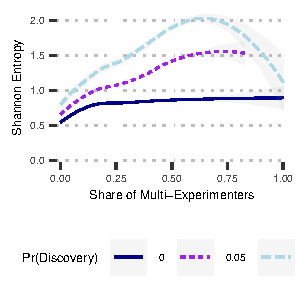
\includegraphics[width=\linewidth]{figures/sim_discovery_shannon.pdf}
        \label{subfig:target_diversity_rob1}
    \end{sublightfigure}
    \begin{sublightfigure}[t]{.3\textwidth}
        \centering
        \caption{}
        \includegraphics[width=\linewidth]{figures/sim_discovery_alo_es.pdf}
        \label{subfig:target_diversity_rob1}
    \end{sublightfigure}
    \begin{sublightfigure}[t]{.3\textwidth}
        \centering
        \caption{}
        \includegraphics[width=\linewidth]{figures/sim_discovery_alo_div.pdf}
        \label{subfig:target_diversity_rob1}
    \end{sublightfigure}
    \begin{sublightfigure}[t]{.3\textwidth}
        \centering
        \caption{}
        \includegraphics[width=\linewidth]{figures/sim_discovery_ss_es.pdf}
        \label{subfig:target_diversity_rob1}
    \end{sublightfigure}
    \begin{sublightfigure}[t]{.3\textwidth}
        \centering
        \caption{}
        \includegraphics[width=\linewidth]{figures/sim_discovery_ss_div.pdf}
        \label{subfig:target_diversity_rob1}
    \end{sublightfigure}
% \caption*{\scriptsize\emph{Notes:} }
\end{lightfigure}



In Figure \ref{fig:appendix_sim_discovery_diversity}, we report simulation results grouped by each discovery probability. In each plot we show binned scatter plots, with 50 bins. We measure the diversity of approaches with Shannon entropy, consistent with our empirical method. In panel (a), our simulations show that the probability of discovery positively moderates the relationship between the share of multi-experimenters and the diversity of approaches. In other words, for a fixed share of multi-experiment firms, when the likelihood of a new approach being discovered is higher, our simulations predict a greater diversity of approaches.

Turning to outcomes, the results are less clear-cut. In panels (b) and (c), we look at the probability of at least one success, and in panels (d) and (e), we look at the average success rate. In panel (b), the simulations suggest a small benefit from discovery on the probability of at least one success. This is consistent with our previous results: a higher discovery rate is associated with a greater diversity of approaches, which is associated with a higher probability of the market finding at least one success. Panel (c) is harder to interpret, but our results suggest a declining benefit to higher discovery rates. Holding the diversity of approaches constant, a higher probability of at least one success is achieved when the discovery rate is lower. 

Panel (d) also conforms with prior results. The share of successful experiments is lower when a market consists of a greater share of multi-experiment firms, especially when the discovery rate is higher. Discovery leads to new approaches becoming available, but individually, they have a smaller probability of success. Panel (e) suggests results consistent with the intuition of the panel (c). Holding the diversity of approaches constant, the share of experimental successes will be lower when the discovery rate is higher.






% \subsection{Extension: Rent Dissipation}


% \begin{lightfigure}[h!]
% \caption{\textsc{Simulating the Effect of Rent Dissipation on the Diversity of Approaches and the Outcomes of Experiments}}
% \label{}
%     \centering
%     \begin{sublightfigure}[t]{.3\textwidth}
%         \centering
%         \caption{}
%         \includegraphics[width=\linewidth]{figures/sim_rentdiss_diversity.pdf}
%         \label{subfig:sim_rentdiss_diversity}
%     \end{sublightfigure}
%     \begin{sublightfigure}[t]{.3\textwidth}
%         \centering
%         \caption{}
%         \includegraphics[width=\linewidth]{figures/sim_rentdiss_success_share.pdf}
%         \label{subfig:sim_rentdiss_success_share}
%     \end{sublightfigure}
%     \begin{sublightfigure}[t]{.3\textwidth}
%         \centering
%         \caption{}
%         \includegraphics[width=\linewidth]{figures/sim_rentdiss_atleastone_on_share.pdf}
%         \label{subfig:sim_rentdiss_atleastone_on_share}
%     \end{sublightfigure}
% \caption*{\scriptsize\emph{Notes:} 
% This simulation uses the following parameters: $\pi_a = 0.4$, $\pi_b = 0.2$, $p_a = p_b = 0.3$.}
% \end{lightfigure}


% \subsection{Extension: Value of Experimentation}

% \begin{lightfigure}[h!]
% \caption{\textsc{Simulating the Effect of Value on the Diversity of Approaches and the Outcomes of Experiments}}
% \label{}
%     \centering
%     \begin{sublightfigure}[t]{.3\textwidth}
%         \centering
%         \caption{}
%         \includegraphics[width=\linewidth]{figures/value_sims_diversity.pdf}
%         \label{subfig:value_sims_diversity}
%     \end{sublightfigure}
%     \begin{sublightfigure}[t]{.3\textwidth}
%         \centering
%         \caption{}
%         \includegraphics[width=\linewidth]{figures/value_sims_success_share.pdf}
%         \label{subfig:value_sims_success_share}
%     \end{sublightfigure}
%     \begin{sublightfigure}[t]{.3\textwidth}
%         \centering
%         \caption{}
%         \includegraphics[width=\linewidth]{figures/value_sims_atleastone_success.pdf}
%         \label{subfig:value_sims_atleastone_success}
%     \end{sublightfigure}
% \caption*{\scriptsize\emph{Notes:} 

% This simulation uses the following parameters: $\pi_a = 0.4$, $\pi_b = 0.2$, $p_a = p_b = 0.3$.}
% \end{lightfigure}

\clearpage
\section{Data}\label{app:data}

\subsection{Description of Variables}

\begin{lighttable}[h!]
    \centering
    \footnotesize
    % \caption{Description of Variables}
    \caption*{\scriptsize\emph{Notes:} All variables are defined at the therapeutic class--year level ($i, t$)}
    \vspace{1em}
    \resizebox{\textwidth}{!}{
        \input{tables/description-of-variables}
    }
    \label{app:description-of-variables}
    \vspace{1em}
\end{lighttable}


\subsection{Matching Pharmaprojects to Pitchbook}\label{app:matching_pharma_to_pitch}

We match data on firm founding year and ownership from Pitchbook to Pharmaprojects by firm name. Matching by firm name is challenging, because datasets often use different naming conventions. For example, one dataset may list ``Eli Lilly \& Co.'', while the other simply states ``Lilly''. Here we briefly describe our approach to this inherently noisy matching task and report results from manual validation.

We first filter firms in Pitchbook by their primary industry group, selecting industries that contain the phrases pharmaceuticals, healthcare, drugs, medical, surgical, hospitals, and clinics. We then clean firm names, removing punctuation, special characters, and common legal suffixes, e.g., ltd., inc., co.

Matching on these cleaned firm names produces multiple matches for each firm in Pharmaprojects. For example, we find that Pfizer matches to many subsidiaries or overseas business units. To identify the focal firm in each match, we keep the matched firm with the oldest founding year. If this data is missing, we select the matched firm with the largest number of employees.

Out of 2,804 pharmaceutical firms, we matched 2,150 to Pitchbook. To validate our match, we took a random sample of 50 firms from those that were matched and another random sample of 50 firms from those that were not matched. For those that were matched, we compared the matches across other observable dimensions, such as HQ location. These manual checks revealed one error in the random sample of 50 firms. As for the unmatched firms, we repeated the same process but with the unfiltered Pitchbook data (i.e., not conditioning on pharmaceutical-relevant firms). For the 654 unmatched firms, we found a match for 76 firms. However, we found that only half of these were accurate upon manual inspection.

In sum, our matching approach is highly accurate, but the main limitation is the coverage of the data.

\subsection{Identifying ATC-1 groups}\label{app:indentify_atc1}

In our analyses, we control for unobserved time and industry varying trends using $ATC1\times{Year}$ fixed effects \citep{branstetter2022generic}. Our data, however, do not include the ATC-1 code to which the therapeutic class belongs. Fortunately, there are only 14 ATC-1 categories (\url{https://www.who.int/tools/atc-ddd-toolkit/atc-classification}). We exclude ATC P: Antiparasitic products, insecticides and repellents, which leaves 13 codes. In a similar approach to matching our sample to GWAS, we loop through our 200 therapeutic class names and use GPT-4.0 to identify the closest ATC-1 match. We match 139 out of 200 therapeutic class designations to an ATC-1 code. Importantly, the therapeutic classes which we match are those pervasive, as we only lose 268 (out of 2,791) observations when we exclude therapeutic classes that we are unable to match to an ATC-1. We ran all of our analyses including these 268 observations grouped under a pseudonym ATC-1 `X'. Though not reported here, all of these results were very similar to those reported in the main paper and this Appendix.

\subsection{Matching Pharmaprojects to GWAS}\label{app:matching_pharma_to_gwas}

%\todo[inline]{GWAS is only for diseases due to genetic mutations - though that might be the bulk of the diseases}

A key feature of our analysis includes controlling for the frequency of discovery. The variable we construct---$\ln$(Discovery)---is the natural logarithm of the number of GWAS publications reporting a new target relevant to therapeutic class $i$ in year $t$. 

Founded in 2008 by the National Human Genome Research Institute, GWAS (\url{https://www.ebi.ac.uk/gwas})---or the Catalog of human Genome-Wide Association Studies---is a record of all scientific publications in top-tier journals reporting the discovery of a new target--disease correspondence. An in-depth overview of GWAS is provided by \citet{tranchero2023finding}. 

\begin{lightfigure}[h!]
\caption{\textsc{New Gene-Disease Discoveries Over Time}}
\label{fig:discovery_over_time}
    \centering
        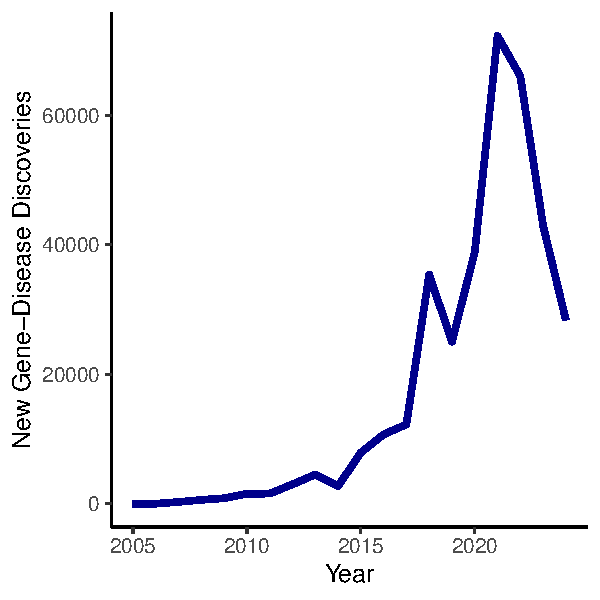
\includegraphics[width=.4\linewidth]{figures/discovery_over_time.pdf}
\end{lightfigure}

The GWAS catalog only reports the disease and/or trait that a particular study is concerned with, so to match these data to Pharmaprojects, we need to make a correspondence between disease/traits and therapeutic class. We create two lists of the 200 distinct therapeutic class names and 28,540 disease names from GWAS. We then wrote a Python script that looped through each disease name and used OpenAI's GPT-4.0 API to identify any and all (at most three) corresponding therapeutic class names. We matched 22,381/28,840 disease names to 179/200 therapeutic classes. Then, for each therapeutic class--year, we count the number of new discoveries in corresponding diseases published in GWAS in that year. As Figure \ref{fig:discovery_over_time} shows, the coverage of GWAS is considerably weaker for the first three-quarters of our sample period (GWAS was only founded in 2008, after all). Consequently, we have a measure of discovery for 811 out of 2791 market observations. After dropping observations where we don't have an ATC-1 code, this becomes 809. 

\clearpage
\section{Robustness Analysis}\label{app:robustness}


%%%%%%%%%%%%%%%%%%%%%%%%%%%%%%%%%%%%%%%%%%%%%%%%%%%%%%%%%%%%%%%%%%%%%%%%%%%
%%%%%%%%%%%%%%%%%%%%%%%%%%%%%%%%%%%%%%%%%%%%%%%%%%%%%%%%%%%%%%%%%%%%%%%%%%%

\begin{lighttable}[h!]
    \centering
    \scriptsize
    \caption{\textsc{Replication of baseline results with unproven targets only}}
    \vspace{1em}
    \centering
            \input{tables/robustness/drop-targets-where-pi-equals-one}
    \vspace{1em}
    \label{app:drop_pi_equal_one}
    \caption*{\scriptsize\emph{Notes:} These table replicate the baseline results from Table \ref{tab:baseline-regressions-all-props}, where the underlying dataset has been modified to exclude projects using targets which have been targeted by at least one launched drug in the same therapeutic class. all models are estimated with OLS. Robust standard errors clustered at the ATC-1 level are shown in parentheses. Significance codes: * p<.1, ** p<.05, *** p<.01 
    }
\end{lighttable}


%%%%%%%%%%%%%%%%%%%%%%%%%%%%%%%%%%%%%%%%%%%%%%%%%%%%%%%%%%%%%%%%%%%%%%%%%%%
%%%%%%%%%%%%%%%%%%%%%%%%%%%%%%%%%%%%%%%%%%%%%%%%%%%%%%%%%%%%%%%%%%%%%%%%%%

\begin{lighttable}[h!]
    \centering
    \scriptsize
    \caption{\textsc{Replication of key results with market defined in longer time windows}}
    \label{app:longer_time_windows}
    \vspace{1em}
    \begin{minipage}{\textwidth}
    \centering
    \caption*{(a) Unit of Observation = Therapeutic Class---Two Year Period}
            \input{tables/robustness/2yearwindow}

  \end{minipage}
    \begin{minipage}{\textwidth}
    \vspace{1em}
    \centering
    \caption*{(b) Unit of Observation = Therapeutic Class---Five Year Period}
            \input{tables/robustness/5yearwindow}
  \end{minipage}
    \vspace{1em}
    \caption*{\scriptsize\emph{Notes:} These table replicate the baseline results from Tables \ref{tab:baseline-regressions-all-props}, where the underlying dataset has been modified to allow for longer time windows. In the original results, we defined the unit of observation---a market---as a therapeutic class--year. In Panel (a), the unit of observation is a therapeutic class--two year period i.e., 1996-1997 is period 1, 1998-1999 is period 2, and so on. In Panel (b), the unit of observation is a therapeutic class--five year period i.e., 1996-2000 is period 1, 2001-2005 is period 2, and so on. Robust standard errors clustered at the ATC-1 level are shown in parentheses. Significance codes: * p<.1, ** p<.05, *** p<.01 
    }
\end{lighttable}



%%%%%%%%%%%%%%%%%%%%%%%%%%%%%%%%%%%%%%%%%%%%%%%%%%%%%%%%%%%%%%%%%%%%%%%%%%%
%%%%%%%%%%%%%%%%%%%%%%%%%%%%%%%%%%%%%%%%%%%%%%%%%%%%%%%%%%%%%%%%%%%%%%%%%%%
%% HHI & DRUG LAUNCH


\begin{lighttable}[h!]
    \centering
    \scriptsize
    \caption{\textsc{Replication of key results with HHI and Drug Launch}}
    \label{app:alternative_measures}
    \vspace{1em}
    \begin{minipage}{\textwidth}
    \centering
    \caption*{(a) Measuring Diversity with HHI}
            \input{tables/robustness/HHI}

  \end{minipage}
    \begin{minipage}{\textwidth}
    \vspace{1em}
    \centering
    \caption*{(b) Measuring Success with Drug Launch}
            \input{tables/robustness/success_as_launch}
  \end{minipage}
    \vspace{1em}
    \caption*{\scriptsize\emph{Notes:} 
    Panel (a) replicates the baseline results from Table \ref{tab:baseline-regressions-all-props}, where the variable Target Diversity has been replaced with HHI. A higher HHI value indicates that experiments are concentrated in a handful of approaches, and thus the market is less diverse. Panel (b) replicates the baseline results from Table \ref{tab:baseline-regressions-all-props} where we define success as a drug development project ultimately leading to a drug product launch. Robust standard errors clustered at the ATC-1 level are shown in parentheses. Significance codes: * p<.1, ** p<.05, *** p<.01 
    }
\end{lighttable}






%%%%%%%%%%%%%%%%%%%%%%%%%%%%%%%%%%%%%%%%%%%%%%%%%%%%%%%%%%%%%%%%%%%%%%%%%%%
%%%%%%%%%%%%%%%%%%%%%%%%%%%%%%%%%%%%%%%%%%%%%%%%%%%%%%%%%%%%%%%%%%%%%%%%%%%
%% 2SLS

\begin{lighttable}[h!]
    \centering
    \scriptsize
    \caption{\textsc{Two-stage least-squares (2SLS)}}
    \vspace{1em}
    \centering
            {
\def\sym#1{\ifmmode^{#1}\else\(^{#1}\)\fi}
\begin{tabular}{l*{2}{c}}
\hline\hline
                                        &\multicolumn{1}{c}{\shortstack{Average\\Experimenter\\Scale (t)}}&\multicolumn{1}{c}{\shortstack{Target\\Diversity}}\\\cmidrule(lr){2-2}\cmidrule(lr){3-3}
                                        &\multicolumn{1}{c}{(1)}&\multicolumn{1}{c}{(2)}\\
                                        &\multicolumn{1}{c}{First Stage}&\multicolumn{1}{c}{2SLS}\\
\hline
Average Experimenter Scale\textsubscript{t-1)}&       0.086\sym{***}&                     \\
                                        &     (0.019)         &                     \\
Average Experimenter Scale              &                     &       1.747\sym{**} \\
                                        &                     &     (0.599)         \\
\hline
Market Structure Controls               &         Yes         &         Yes         \\
ATC-1$\times$Year FE                    &         Yes         &         Yes         \\
Observations                            &       2,362         &       2,362         \\
Adj R-squared                           &       0.271         &       0.564         \\
First Stage F-test                      &                     &      39.559         \\
\hline\hline
\end{tabular}
}

    \vspace{1em}
    \label{app:2sls}
    \caption*{\scriptsize\emph{Notes:} This table replicate the baseline results from column (2) of Table \ref{tab:baseline-regressions-all-props}, using lagged experimenter scale as an instrument. Robust standard errors clustered at the ATC-1 level are shown in parentheses. Significance codes: * p<.1, ** p<.05, *** p<.01 
    }
\end{lighttable}





% \begin{lightfigure}[h!]
% \caption{A DAG motivating our 2SLS instrumental variable design}
%         \centering
%         \includegraphics[width=\linewidth]{figures/2sls-dag.pdf} 
% \label{fig:dag}
% \end{lightfigure}
\clearpage


\end{document}

